\documentclass[11pt]{article} 
\usepackage[american]{babel}
\usepackage{makeidx}
\usepackage{amssymb}
\usepackage{amsmath}
\usepackage{xfrac}
\usepackage{graphicx}
\usepackage{amsthm}
\usepackage{caption}
\usepackage{subcaption}
\usepackage{enumerate}
\usepackage{enumitem}

\oddsidemargin= -12pt \evensidemargin= -12pt
\topmargin=-45pt
\binoppenalty=10000
\relpenalty=10000
\textwidth=6.5in\textheight=9in \baselineskip=18pt
\parskip=6pt plus 1pt
\numberwithin{equation}{section}

\newtheorem{proposition}{Proposition}[section]
\newtheorem{lemma}{Lemma}[proposition]
\newcommand{\pr}{{\rm Pr}}
\newcommand{\e}{{\rm E}}
\newcommand{\expdist}{{\rm exp}}
\newcommand{\U}{{\rm U}}
\DeclareMathOperator*{\argmin}{arg\,min}

\begin{document}

\begin{center} \Large {\bf Strategic Sensing in Cognitive Radio Networks}
\end{center}

\begin{abstract} 

We study a noncooperative multi-player game problem of individual rational users sending data-packets (``customers'' in the terminology of queueing theory) in a Cognitive Radio Network (CRN) with the opportunity of spectrum sensing. The system is composed of two channels (or ``servers''): One unlicensed channel shared freely among all users, and one in which the transmission entails the cost of sensing, and can be denied if the channel is already occupied. It is the users' prerogative to decide whether to use the shared channel or sense, hopefully not encountering a rejection. If a denied customer leaves never to return, the system can be analyzed as two independent subsystems with poissonian stream of arrivals to each one, an M/M/1/1 and an M/M/1, and it can be easily shown that that there exists a unique Nash equilibrium. As opposed to such simple models, in our model customers that are rejected from service after sensing are routed to the shared queue. We model this process as a queueing system comprising of two servers working in parallel, one is an M/M/1/1 loss system and the other is a G/M/1 with heterogeneous arrivals. We compute the transition probabilities and the stationary probabilities of the Markov chain describing the process, analyze the system's capacity and utilization and show, using the technique of Sample Path Analysis, that the Nash equilibrium strategy in the system is well-defined.

\newpage

\end{abstract}

\section{Introduction}

\newpage

\section{System-model}

We consider a system composed of two identical servers, $S_Q$ and $S_L$ (Q for queue, L for loss), each one's service-duration is exponential with rate $\mu$, and a single FCFS unobservable queue (see Fig.\ref{CustomersFlow}). Customers are identical, and arrive at the system following a Poisson process with rate $\Lambda$. Upon arrival, a costumer chooses one of two options: pay a {\it sensing price} and try to attain service in $S_L$ (a.k.a, {\it Sense}), or join the queue and wait until accepted to service in $S_Q$. A costumer who chooses to sense $S_L$ and finds it idle is immediately accepted to service without waiting. If he/she finds $S_L$ occupied, he/she is sent to the queue and waits his/her turn to service by $S_Q$.

Denote $p$ the probability that a costumer senses $S_L$, and denote $(X(t), Y(t))$ the state of the system at time $t$, consisting of $X(t) \in \lbrace0, 1, 2, \ldots\rbrace$ the number of customers in the queue (including the one in service at $S_Q$), and $Y(t) \in \lbrace0, 1\rbrace$ the state of $S_L$ (where $Y(t)=0$ means that $S_L$ is idle at time $t$). Thus, the system can be described as a bi-dimensional Markov process, as shown in Fig.\ref{MarkovChain}, and the stationary probabilities are computed through the following set of equations: 

\begin{equation}
  \begin{cases}
    \Lambda P_{0,0} - \mu P_{1,0}  - \mu P_{0,1} = 0\:,\\
    (\mu+\Lambda) P_{0,1} - p\Lambda P_{0,0}  - \mu P_{1,1} = 0\:.
  \end{cases}
	\label{StateEq1}
\end{equation}

\begin{equation}
  \forall n \in \lbrace 1, 2, \ldots \rbrace: \ \begin{cases}
    (\mu+\Lambda) P_{n,0} - (1-p) \Lambda P_{n-1, 0} - \mu P_{n+1,0}  - \mu P_{n,1} = 0\:,\\
    (2\mu+\Lambda) P_{n,1} - p\Lambda P_{n,0}  - \Lambda P_{n-1,1} - \mu P_{n+1,1} = 0\:.
  \end{cases} \label{StateEq2}
\end{equation}
where $P_{i,j}$ is the stationary probability that the system is in state $(i,j)$. These equations lead to the following relationship:

\begin{equation}
  \forall n \in \lbrace 0, 1, 2, \ldots \rbrace: \ 
    P_{n+1,0} + P_{n+1,1} = \dfrac{\Lambda}{\mu}((1-p) P_{n,0} + P_{n, 1})\:, \label{RecurtionRule}
\end{equation}

By the assumption that each individual chooses randomly and independently whether or not to sense, we deduce that the sub-system $S_L$ can be considered as an M/M/1/1 queue (Erlang's Loss Model) with arrival rate $p\Lambda$ and service rate $\mu$. Therefore, the {\it loss-probability} of $S_L$ (i.e., the probability that a customer sensing $S_L$ will find it occupied) is:
\begin{equation}
	\pr(Y=1) = \sum\limits_{i=0}^{\infty} P_{i, 1} = \dfrac{p\Lambda}{\mu+p\Lambda}\:, \label{LossProb}
\end{equation}
and its complement:
\begin{equation}
	\pr(Y=0) = 1-\pr(Y=1) = \sum\limits_{i=0}^{\infty} P_{i, 0} = \dfrac{\mu}{\mu+p\Lambda}\:. \label{OMLossProb}
\end{equation}
One can also derive the above formula by summing the right-hand-sides of the equations in (\ref{RecurtionRule}) for $n=0,1,2,\ldots$ and equating the sum of this infinite series to $1-(P_{0,0}+P_{0,1})$, considering that in steady state of the system: \[ p\Lambda\sum_{i=0}^{\infty}P_{i,0} - \mu \sum_{i=0}^{\infty}P_{i,1} = 0\:.\]

Summing the equations in (\ref{RecurtionRule}) for $n=0,1,2,\ldots$ and utilizing (\ref{LossProb}) and (\ref{OMLossProb}) we get:

\begin{equation}
	P_{0,0} + P_{1,0} = 1- \frac{ \Lambda}{ \mu}\left(1- \frac{p}{1+p \frac{\Lambda}{\mu}} \right) \label{P00PlusP01}
\end{equation}
which induces a linear relationship between $P_{0,0}$ and $P_{0,1}$.

Subtracting the second equation from the first one in (\ref{StateEq2}) and combining with (\ref{RecurtionRule}) we deduce the following formulae:
\begin{equation}
	\forall n \in \lbrace 0, 1, \ldots \rbrace: \
  	\begin{cases}
    	P_{n+1,0} = (1-p) \frac{\Lambda}{\mu} P_{n, 0} + p \frac{\Lambda}{\mu} \sum\limits_{i=0}^{n}P_{i,0} - \sum\limits_{i=0}^{n}P_{i,1}\:, \\
   	 	P_{n+1,1} = \frac{\Lambda}{\mu} P_{n, 1} + \sum\limits_{i=0}^{n}P_{i,1} - p \frac{\Lambda}{\mu} \sum\limits_{i=0}^{n}P_{i,0} \:.
  	\end{cases} \label{Forms}
\end{equation}
It can be seen from (\ref{Forms}) that, for given constants $p$ and $\sfrac{\Lambda}{\mu}$, every value $P_{n+1,k}$ ($k\in\lbrace0,1\rbrace$) is expressed as a linear combination of $\lbrace P_{0,0}, P_{1,0}, \ldots, P_{n,0}, P_{0,1}, P_{1,1}, \ldots, P_{n,1}  \rbrace$. Hence, with (\ref{P00PlusP01}), it follows by induction that for each $n \in \lbrace 0, 1, \ldots \rbrace$ and for each $k \in \lbrace 0, 1 \rbrace$, $P_{n,k}$ is a linear function of $P_{0,0}$, as a countable sum of linear functions. Thus, for $N$ sufficiently large, one can bound the queue length by $N$, express the finite series $\sum_{i=0}^{N} P_{i,0}+P_{i,1}$ as a linear function of $P_{0,0}$, equate to 1 and find a fixed value of $P_{0,0}$ (and all other $P_{n,k}$) in $O(N)$ time complexity.
\newpage

\section{System-utilization}
We now intend to find the maximum utilization of the system. For convenience we use the notation $\rho:=\sfrac{\Lambda}{\mu}$. The {\it effective-arrival-rate} to the queue, $\hat{\lambda}(p,\rho)$, consists of two streams of arrivals: customers who join the queue without sensing at all (whose proportion is $1-p$) and customers who sense $S_L$ and find it busy (whose proportion is $p \cdot \pr(Y=1)$). Therefore,
\[ \hat{\lambda}(p,\rho) = (1-p)\Lambda + \pr(Y=1)\cdot p \Lambda \:. \]
Using (\ref{LossProb}) and dividing by $\mu$ we get the {\it effective-utilization}, $\hat{\rho}(p,\rho)$:
\begin{equation}
\hat{\rho}(p,\rho) := \frac{1}{\mu}\hat{\lambda}(p,\rho) = \rho - p\rho + \frac{p\rho}{1+p\rho}p\rho = \rho - \frac{1}{1+p\rho}p\rho\:, \label{EffectiveUtil}
\end{equation}
which is monotone decreasing in $p$ for every $\rho\in(0,\infty)$. 

Note, by (\ref{P00PlusP01}), that $\hat{\rho}(p,\rho)$ is equal to $1-(P_{0,0}+P_{0,1})$, for it represents the {\it busy fraction} of subsystem $S_Q$.

The stochastic process representing the stream of arrivals over time to the queue served by $S_Q$ is not necessarily poissonian. This is because the inter-arrival times to the queue for $p \neq 0$ are not i.i.d., and the arrival-rate increases when $S_L$ is busy in comparison to the arrival-rate in its idle periods. Thus, we model this subsystem as a G/M/1 with heterogeneous inter-arrival times, and for the system to remain stable, as implied by \cite{Yehiali&Naor}, we assume $\hat{\rho}(p,\rho) < 1$.

Recall the {\it golden ratio}, $\varphi = \sfrac{1}{2} \cdot (1+\sqrt{5})\approx 1.618$. Then:

\begin{proposition}
For each $\rho\in(0,\varphi)$, there exists a lower bound for $p$, denoted $\underline{p}$, such that the system is stable iff $p \in (\underline{p}, 1]$.
\end{proposition}

\begin{proof}
As discussed, a necessary and sufficient condition for stability is: $\hat{\rho}(p,\rho) < 1$. Substitute (\ref{EffectiveUtil}) and isolate $p$ in the inequality to get an equivalent stability criterion:
\[ p > \frac{\rho - 1}{\rho(2-\rho)} =: \underline{p}\]
from which it is clear that, if the system is stable for some $p_0 > \underline{p}$, it is also stable for all $p \in [p_0,1]$.

Finding the maximum throughput we assume that $p=1$, which means everyone senses $S_L$ before they join the queue. This is followed by the monotonicity of $\hat{\rho}(p,\rho)$. Then, from (\ref{EffectiveUtil}), the stability criterion is:
\[ \hat{\rho}(1,\rho)=\frac{\rho^2}{1+\rho}<1 \quad\Leftrightarrow\quad \rho^2-\rho-1<0 \quad\Leftrightarrow\quad \rho < \frac{1+\sqrt{5}}{2}=\varphi \]
where $\varphi$ is the golden ratio, concluding that for every $\rho\in(0,\varphi)$ and $p \in (\underline{p},1]$, the system is stable.
\end{proof}

\newpage
\section{Equilibrium Strategy}
In this section we discuss the states and (Nash) equilibrium strategies in the system. Let $c_{w}>0$ be the waiting cost per unit time of an individual customer waiting in line, and $c_{s}>0$ be the cost of sensing (incurred by each customer who chooses to sense, regardless of the consequences of his action). Since all customers are identical, and each one arriving at the system is eventually attained to service, neither the reward from service nor the time spent in service is relevant. Of course, the state of the system, including the length of the queue and the status of the servers, is unobservable as mentioned, and unknown to the customers at the time they make their decisions. We assume the system is not overloaded (i.e., $\rho<\varphi$) and that all customers act to reduce their expected cost to minimum. Denote $C_{S}(p)$ and $C_{N}(p)$ the expected cost of an individual who chooses to sense and an individual who chooses not to sense, respectively, given that the others' probability of sensing is $p$.
\begin{equation}\begin{cases}
 	C_{N}(p) = \frac{c_{w}}{\mu}\e\left[L(p)\right] \:, \\
	C_{S}(p) = c_{s} + \pr(Y=1) \cdot \frac{c_{w}}{\mu} \e\left[L(p)\mid Y=1\right] \:,
\end{cases}
\label{CostFunc}
\end{equation}
where $L(p)$ is a random variable representing the queue length (including the customer in service) upon arrival to the system. 

Prior to discussion of equilibrium strategies we assert some attributes of $\e\left[L(p)\mid Y=0\right]$ which appear to be essential in this context. 
%The claim that this function is non-increasing in $p$ may seem obvious at first glance, as the effective utilization of the queue, $\hat{\rho}(p,\rho)$, defined in (\ref{EffectiveUtil}), is monotone decreasing in $p$. Subsequent glances, however, 

\begin{proposition}
The function $\e\left[L(p)\mid Y=0\right]$ is continuous and monotone non-increasing in $p$. \label{MonotonicityProp}
\end{proposition}

\begin{proof}
Proving the continuity of $\e\left[L(p)\mid Y=0\right]$ is immediate, as, referring to (\ref{OMLossProb}), (\ref{P00PlusP01}) and (\ref{Forms}),
\[ \e\left[L(p)\mid Y=0\right] = \frac{1}{\Pr(Y=0)}\sum\limits_{i=0}^{\infty} i P_{i, 0} = (1+p\rho) \sum\limits_{i=0}^{\infty} i P_{i, 0} \:,\]
which is a countable sum of compositions of continuous functions in $p \in [0,1]$. 

In order to prove monotonicity, we examine the transitions between states in two systems, $\Omega := \lbrace S_Q, S_L \rbrace$ and $\Omega' := \lbrace S'_Q, S'_L \rbrace$, under the same sequence of events. Systems $\Omega$ and $\Omega'$ are identical except that in $\Omega$ the sensing probability is $p$, as opposed to $\Omega'$, where the sensing probability is $p'$, and $p < p'$. 

Denote by $(X(t),Y(t))$ and $(X'(t),Y'(t))$ the states at time $t$ of systems $\Omega$ and $\Omega'$ respectively. Since that for all $p \in [0,1]$ the state $(0,0)$ in the Markov chain is recurrent, we can assume without loss of generality, that at time $t=0$, 
\[(X(0),Y(0)) = (X'(0),Y'(0)) = (0,0)\:.\] 
Showing that 
\begin{equation}
\forall t \in [0,\infty) : \e[X(t) \mid Y(t) = 0] \geq \e[X'(t) \mid Y'(t) = 0] \label{SuffArg4.1}
\end{equation}
will complete the proof.

We begin by attaching three variables to each customer: Let $\lbrace{ (T_i, \tau_i, u_i) \rbrace}_{i \in \mathbb{N} }$ represent the {\it arrival time}, {\it service duration} and {\it sensing aversion} of the $i$-th customer respectively, and for all $i \in \mathbb{N}$: 
\[T_{i+1} - T_i \sim \expdist(\Lambda) \:, 
\quad \tau_i \sim \expdist(\mu) \:,
\quad u_i \sim \U[0,1] \:.\]
Each customer arrives to both systems simultaneously. Customer $i$ arriving at $\Omega$ senses if and only if $u_i \leq p$, and similarly, arriving at $\Omega'$ he/she senses if and only if $u_i \leq p'$. This ensures that the sensing probability is $p$ in system $\Omega$ and $p'$ in system $\Omega'$, and as a fact, implies that customers who sense in $\Omega$ also sense in $\Omega'$. Note that the value $u_i$ is only relevant when 
$Y(T_i)=0$ or $Y'(T_i)=0$.

We assign each customer one of three types, based on the values of their sensing aversion: Customer $i$ will be assigned
\begin{itemize}
\item {\it type-L} (stands for ``Low'') if $u_i \in [0, p]$,
\item {\it type-M} (stands for ``Medium'') if $u_i \in (p, p']$,
\item {\it type-H} (stands for ``High'') if $u_i \in (p',1]$.
\end{itemize}
We reiterate that one's type is only significant if $S_L$ or $S'_L$ are empty by the time of customers' arrival.
By definition, upon arrival, an H-type customer joins both $S_Q$ and $S'_Q$, an M-type customer joins $S_Q$ but senses $S'_L$, whereas an L-type customer senses both $S_L$ and $S'_L$.

Without loss of generality, we modify the service regime as follows: 
\begin{enumerate}[label=(\roman*)]
\item\label{Assump1} Arriving at $\Omega$ ($\Omega'$) when $S_L$ ($S'_L$) is busy, customer $i$ preempts the customer in service in $S_L$ ($S'_L$) with no regard to type, and the preempted customer is routed to continue the service in $S_Q$ ($S'_Q$). Arriving at $\Omega$ ($\Omega'$) when $S_L$ ($S'_L$) is empty, customer-$i$'s actions are followed by type.
\item\label{Assump2} Subsystem $S_Q$ ($S'_Q$) is a preemptive resume LCFS queue, meaning that customers are served following a preemptive LCFS discipline, and the preempted service will be resumed from the point it is stopped.
\end{enumerate}

\begin{lemma}
Assumptions {\rm \ref{Assump1}} and {\rm \ref{Assump2}} do not affect the stationary probabilities of the systems. \label{WlogAssump}
\end{lemma}

\begin{proof}

We shall show that Lemma \ref{WlogAssump} holds for system $\Omega$ and the proof for $\Omega'$ is identical. 

Let $i$ and $i+1$ be a successive pair of customers and suppose that customer $i+1$ preempts customer $i$ in subsystem $S_L$. Denote $\Delta_{i,i+1} := T_{i+1}-T_i$ the time difference between their arrivals. Then, as a result of the memoryless property of the exponential distribution, the service duration of customer $i+1$ (i.e., $\tau_{i+1}$) and the residual service of customer $i$ (i.e., $\tau_i-\Delta_{i,i+1} \mid \tau_i>\Delta_{i,i+1}$) are independent and identically distributed. This incident of preemption is equivalent to the joining of the new comer to  subsystem $S_Q$ when $S_L$ is busy. Hence, assumptions \ref{Assump1} does not influence the transition probabilities and the stationary probabilities remain as before.

The validity of assumption (ii) can be explained by the fact that in a work-conserving preemptive resume system with exponential i.i.d services duration, as sustains in $S_Q$, the length of the queue is independent of the service regime. Consequently, assumptions \ref{Assump1} and (ii) do not restrict the generality of the model.
\end{proof}

Exploiting assumptions \ref{Assump1} and \ref{Assump2} we immediately achieve several properties that will be later used in the proof:

\begin{lemma}
Under assumptions {\rm \ref{Assump1}} and {\rm\ref{Assump2}}, the following arguments hold:

\begin{enumerate}[label=(\alph*)]
\rm \item\label{Prop1} \it At any moment, if $S_L$ ($S'_L$) is not idle, then the last customer to arrive until that moment is in $S_L$ ($S'_L$).
\rm \item\label{Prop2} \it All customers begin service at the moment of their arrival, whether they sense or not.
\rm \item\label{Prop3} \it Customers joining $S_L$ upon their arrival,  attend $S'_L$ as well.
\rm \item\label{Prop4} \it Customers joining $S'_Q$ upon their arrival, attend $S_Q$ as well.% (the {\it modus tollens} form of \ref{Prop3}).
\rm \item\label{Prop5} \it The sojourn time of customer $i$ in $S'_Q$ is no greater then the sojourn time of $i$ in $S_Q$.% (from \ref{Prop4}, customers who arrive at $S'_Q$ after $i$, simultaneously arrive at $S_Q$).

\end{enumerate}
\end{lemma}

\begin{proof}
\begin{enumerate}[label=(\alph*)]
\item From assumption \ref{Assump1}, in a certain time $t$, the only scenario in which the last customer to arrive at $\Omega$ does not join $S_L$, is when he/she is not of type 'L' and $S_L$ is idle at the moment of his/her arrival. Hence, $S_L$ stays idle at time $t$. The proof for $\Omega'$ is similar.
\item At the moment of their arrival, costumers either begin service immediately in $S_L$, or, by assumption \ref{Assump2} join the head of the line in $S_Q$. The proof for $\Omega'$ is similar.
\item Recall that at time $t=0$ both $S_L$ and $S'_L$ are empty. Only upon an arrival of an L-type customer will the state of $S_L$ alter. Arriving at $\Omega'$, an L-type customer joins $S'_L$, regardless of the server's state. Suppose the last customer has joined both $S_L$ and $S'_L$. By assumption \ref{Assump1}, this tagged customer can either complete service in $S_L$ and $S'_L$ simultaneously (so $S_L$ and $S'_L$ become empty) or be preempted in the two subsystems by the next customer to come. As for the latter case, it holds that the preempting customer joins both $S_L$ and $S'_L$. Thus, it follows by induction that customers who join $S_L$ also join $S'_L$.
\item This property is immediately achieved as the {\it modus tollens} form of property \ref{Prop3}.
\item It results from assumption \ref{Assump2} that the sojourn time of each customers depends on future arrivals to the queue. Combining this with property \ref{Prop4} we deduce \ref{Prop5}. 
\end{enumerate}
\end{proof}

With property \ref{Prop3} and the simultaneousness of occurrences we get:
\[ \forall t  \in [0, \infty): \lbrace{ Y(t)=1 \rbrace} \Rightarrow \lbrace{ Y'(t)=1 \rbrace} \:, \]
or, in an analogous fashion:
\begin{equation}
\forall t  \in [0, \infty): \lbrace{ Y'(t)=0 \rbrace} \Rightarrow \lbrace{ Y(t)=0 \rbrace} \:.\label{BusyTimesComp}
\end{equation}
Moreover, from properties \ref{Prop4} and \ref{Prop5}, we see that at an arbitrary point in time, each customer in $S'_Q$, must as well linger in $S_Q$, not leaving $\Omega$ before leaving $\Omega'$. Therefore, 
\begin{equation}
\forall t \in [0, \infty):  X(t) \geq X'(t) \:, \label{StDomination}
\end{equation}
which implies that the process representing the number of customers in $S_Q$ over time stochastically dominates the one that represents the number of customers in $S'_Q$. 

For simplicity, we denote $(X(t), Y(t))$ by $(X,Y)$, and $(X'(t),Y'(t))$ by $(X', Y')$ (all equations are to be understood at an arbitrary time sample). On utilizing (\ref{StDomination}), we get
\[ \e[X' \mid Y' = 0] \leq \e[X \mid Y' = 0] \:.\]
To prove our claim (\ref{SuffArg4.1}) it suffices to prove:
\begin{equation}
\e[X \mid Y' = 0] \leq \e[X \mid Y = 0] \:. \label{SufArg}
\end{equation}

Denote $i$ the last customer that arrived by time $t$, and let \[A(t):= \lbrace \mbox{$i$ joined $S_Q$ and $T_i + \tau_i > t$} \rbrace\]
express the event ``$i$ joined $S_Q$ and had not left until $t$''. Because of property \ref{Prop2}, this is possible if and only if $i$ was still in service in $S_Q$ by time $t$. By definition,
\begin{equation}
A(t) \Rightarrow \lbrace Y(t)=0 \rbrace \:. \label{ZCausesY0}
\end{equation}
Clearly, given that $i$ has not left $\Omega$ by time $t$, the residual service of customer $i$ at $t$ is exponential with parameter $\mu$. Thus, we can assume w.l.o.g that $T_i$ occurred a moment before $t$ and $A(t)$ can be rewritten as the event when a new busy period in $S_Q$ began right before $t$ (i.e., $t = T_i^+ := T_i +\varepsilon$, where $\varepsilon$ is a small positive infinitesimal quantity).

Recall that, by property \ref{Prop1}, if there is a customer in $S_L$ at time $t$, then it must be $i$ (the last customer arrived). So, if $t \in \mathbb{R}$ satisfies $Y(t)=0$ and $Y'(t)=1$, customer $i$ joined $S_Q$ at the same time beginning service in $S'_L$, and, together with property \ref{Prop2}, had not left the system before $t$. Hence,
\begin{equation}
\lbrace \lbrace Y'(t)=1 \rbrace \wedge \lbrace Y(t)=0 \rbrace \rbrace \Rightarrow A(t) \:. \label{Y'1&Y0ImplZ}
\end{equation}

\begin{lemma}
Conditioned on $A(t)$, $X(t)$ and $Y'(t)$ are independent random variables.
\label{CondIndep}
\end{lemma}
\begin{proof}
Denote $T_n^+$ the moment after customer-$n$'s arrival. We shall show by induction that $\forall n \in \mathbb{N}$, $ X(T_n^+)$ and $Y'(T_n^+)$ are conditionally independent given $A(T_n^+)$.

Note that as $A(T_n^+)$ occurs, the values of $Y'(T_n^+)$ can be specified one to one by customer-$n$'s actions: 
\begin{equation}
\lbrace Y'(T_n^+) \mid A(T_n^+) \rbrace = \begin{cases} 0, \mbox{ iff $n$ joins $S'_Q$}; \\ 1, \mbox{ iff $n$ joins $S'_L$}. \end{cases}\label{Y'(Tn+)|A(Tn+)}
 \end{equation}

Presume that $A(T_n^+)$ is satisfied. Having that $n$ joined $S_Q$ means that $n$ is not of type-L, and, by (\ref{ZCausesY0}), $Y(T_n^+)=0$. Define $T_i^- := T_i -\varepsilon$, where $\varepsilon$ is a small positive infinitesimal quantity, the moment before $i$'s arrival. Regarding $n$'s arrival at $\Omega'$, there are two possibilities:
\begin{itemize}
\item Upon $n$'s arrival, $S'_L$ was empty (i.e., $Y'(T_n^-)=0$).
\item Upon $n$'s arrival, $S'_L$ was busy (i.e., $Y'(T_n^-)=1$).
\end{itemize}

To the extent that $Y'(T_n^-)=0$, $n$'s action is determined by type (M or H), which is chosen randomly and independently, thus (\ref{Y'(Tn+)|A(Tn+)}) can be rephrased to
\[
\lbrace Y'(T_n^+) \mid A(T_n^+) \rbrace = \begin{cases} 0, \mbox{ iff $n$ is of type-H}; \\ 1, \mbox{ iff $n$ is of type-M}. \end{cases}
\]
and $X(T_n^+)$ and $Y'(T_n^+)$ are independent.

To the extent that $Y'(T_n^-)=1$, then, with assumption \ref{Assump1}, $n$ must have preempted his/her predecessor ($n-1$) in $S'_L$ simultaneously as joining $S_Q$. This is possible only as customer $n-1$ remained in service until customer-$n$'s arrival, and indicates that
\begin{itemize}
\item Customer $n-1$ joined $S_Q$ as arriving at $\Omega$, and $Y(T_{n-1}^+)=0$.
\item Customer $n-1$ joined $S'_L$ as arriving at $\Omega'$, and $Y'(T_{n-1}^+)=Y'(T_n^+)=1$.
\item Customer $n$ had arrived before $n-1$ left $S_Q$, and $X(T_n^+) = X(T_{n-1}^+) + 1$.
\end{itemize}
Supported by the first two statements and (\ref{Y'1&Y0ImplZ}) we infer that $A(T_{n-1}^+)$ holds. Followed by the induction hypothesis, $X(T_{n-1}^+)$ and $Y'(T_{n-1}^+)$ are independent under these conditions, and combining the second and the third statements we deduce that $X(T_{n}^+)$ and $Y'(T_{n}^+)$ are also independent.

It is left to show that $X(T_1^+)$ and $Y'(T_1^+)$ are conditionally independent given $A(T_1^+)$. We can assume, w.l.o.g, that $Y'(T_1)=0$ (otherwise we will observe the last customer that arrived before $T_1$). Thus, as discussed, cusotmer-1's action is equivalent to type, which is a random variable independent of $X(T_1^+)$.
\end{proof}

Define operator $\e_{Y=0}[\bullet] := \e[\bullet \mid Y=0]$.
Combining Lemma \ref{CondIndep} with (\ref{Y'1&Y0ImplZ}), we arrive at
\begin{equation}
\e_{Y=0}[X \mid A] = \e_{Y=0}[X \mid A , Y'=1] = \e_{Y=0}[X \mid Y'=1] \:, \label{IneqZ}
\end{equation}
and since
\[ \e_{Y=0}[X] \leq \e_{Y=0}[X \mid A] \:,\]
upon substituting (\ref{IneqZ}) we get
\begin{equation}
\e_{Y=0}[X] \leq \e_{Y=0}[X \mid Y'=1] \:. \label{E0XleqE0XY'1}
\end{equation}

By the law of total expectation we have
\begin{equation}
\begin{split}
\e_{Y=0}[X] \: = \: & \e_{Y=0}[X \mid Y' = 0]\cdot \Pr(Y' = 0 \mid Y=0) \: +\\ 
& \e_{Y=0}[X \mid Y' = 1]\cdot \Pr(Y' = 1 \mid Y=0) \\
= \: & \e[X \mid Y' = 0]\cdot \Pr(Y' = 0 \mid Y=0) \: +\\ 
& \e_{Y=0}[X \mid Y' = 1]\cdot \Pr(Y' = 1 \mid Y=0)
\:, \label{TotalExpec}
\end{split}
\end{equation}
where the second equality evolves from (\ref{BusyTimesComp}). Let us mention that the right-hand side of (\ref{TotalExpec}) is a convex combination of $\e[X \mid Y' = 0]$ and $\e_{Y=0}[X \mid Y' = 1]$. Amalgamating (\ref{E0XleqE0XY'1}) and (\ref{TotalExpec}) we attain
\[ \e[X \mid Y'=0] \leq \e_{Y=0}[X] \]
thus, confirming (\ref{SufArg}) to complete the proof of Proposition \ref{MonotonicityProp}.
\end{proof}

Denote $\gamma :=\sfrac{c_{w}}{\mu c_{s}}$. The value of $\sfrac{1}{\gamma}$ can be interpreted as the normalized cost of sensing in terms of the cost of waiting a single service period, that is to say, for how many service completions one has to wait, on average, in order to pay a total time expense of $c_{s}$. Then:

\begin{proposition} For every $\rho\in(0,\varphi)$, and for every value $\gamma>0$, a unique equilibrium strategy $p_{e}\in[0,1]$ exists.
\end{proposition}

\begin{proof}

$p$ is an equilibrium strategy if no individual can benefit from choosing any alternative strategy. Thus, for $p \in (0,1)$ to be an equilibrium, the following criterion must hold: 
\begin{equation}
C_{N}(p)=C_{S}(p)\:. \label{EqCriterion}
\end{equation}
Note that:
\[ \e\left[L(p)\right] = \pr(Y=1) \cdot \e\left[L(p)\mid Y=1\right] + \pr(Y=0) \cdot \e\left[L(p)\mid Y=0\right] \:. \]
Divide both sides of (\ref{EqCriterion}) by $c_{s}$ and substitute the values in (\ref{CostFunc}), concluding that for $p \in (0,1)$, $p_{e} = p$ if and only if:
\begin{equation}
\gamma \pr(Y=0) \cdot \e\left[L(p)\mid Y=0\right] = 1\:,
\label{gamma p0 e0 = 1}
\end{equation}
or,
\begin{equation}
\gamma \e\left[L(p)\mid Y=0\right]=1+p\rho\:. \label{EqExistCriterion}
\end{equation}

Note that the function $1+p\rho$ is continuous and strictly monotone increasing in $p$, and therefore, using Proposition \ref{MonotonicityProp}, we deduce that if there exists a solution $p^*$ to (\ref{EqExistCriterion}) then it is unique, and $p_e = p^*$ is a unique equilibrium strategy. 

Suppose that:
\begin{equation}
\forall p \in (0,1): \gamma \e\left[L(p)\mid Y=0\right] > 1+p\rho \:. \label{E0 grt 1+p*rho}
\end{equation}
Following Proposition \ref{MonotonicityProp} and the monotonicity of $1+p\rho$, this inequality holds if and only if \[ \gamma \e\left[L(1)\mid Y=0\right] \geq 1+\rho \:,\] or equivalently: $C_{N}(1) \geq C_{S}(1)$. This means that $p_{e}=1$, and followed by (\ref{E0 grt 1+p*rho}), sensing is a dominant strategy for each individual, and therefore the equilibrium is unique. Similarly, if: 
\[ \forall p \in (0,1): \gamma \e\left[L(p)\mid Y=0\right] < 1+p\rho \] 
then $C_{N}(0) \leq C_{S}(0)$, and $p_{e}=0$, which is unique.
\end{proof}

This result is not as intuitive as it seems, since the function $C_{S}(p)$ is not necessarily monotonic (as shown in Fig. \ref{cost_vs_p_1_0_45} and \ref{cost_vs_p_1_0_725}). This fact can be explained as follows: an increase in the proportion of customers that sense, results in a decrease of the probability to attain service in $S_L$ on the first hand. It also decreases the expected queue length, and shortens the waiting time of the customers who failed to attain $S_L$ on the other hand. Nevertheless, the equilibrium probability $p_{e}$ is always unique.

\begin{proposition}
The pure strategy $p=0$ is an equilibrium strategy (in other words $p_e=0$) iff:
\[ \rho \leq \frac{1}{1+\gamma} \:.\]
\label{p_e=0 condition}
\end{proposition}
\begin{proof}
Assuming that $\hat{\rho}(0,\rho) = \rho < 1$, from (\ref{EqCriterion}), $p=0$ is an equilibrium strategy if and only if:
\[ \gamma \e[L(0)\mid Y=0] \leq 1 \:.\]
Note that in this case the queue is a regular M/M/1 queue, and 
\[ \e[L(0)\mid Y=0] = \e[L(0)] = \frac{\rho}{1-\rho} \:.\] 
Thus, a necessary and sufficient condition for $p_{e}=0$ is:

\[ \gamma \frac{\rho}{1-\rho} \leq 1 \quad\Leftrightarrow\quad \rho \leq \frac{1}{1+\gamma} \:.\]
\end{proof}

\begin{proposition}
The pure strategy $p=1$ is an equilibrium strategy (in other words $p_e=1$) iff:
\[ \theta^4 + (\gamma-1)\theta^3 - (\gamma+1)\theta^2 - \gamma\theta + \gamma \geq 0 \:,\]
which is equivalent to:
\[ \gamma \geq \frac{\theta^2 + \theta^3 - \theta^4}{1- \theta - \theta^2 + \theta^3} \] 
where $\theta := \sqrt{1+\rho}$. \label{p_e=1 condition}
\end{proposition}
\begin{proof}
technical...
\end{proof}

\begin{proposition}
In the particular case $\rho=1$, the following equality holds:
\[ \e[L(p) \mid Y=0] = \frac{1}{p} \:,\]
and
\[ p_e = \min\left\lbrace\frac{\sqrt{1+4\gamma}-1}{2}, 1\right\rbrace \:.\]
\end{proposition}
\begin{proof}
technical...
\end{proof}

\newpage
\section{Social Optimization}

Hereupon, we turn our attention to social optimization. The social objective function, $C(p)$, is defined as 
\begin{equation}
C(p) := (1-p)C_N(p)+pC_S(p) \:, \label{Cp def.}
\end{equation}
and represents the average cost of a customer, where the population's probability of sensing is $p$. Using (\ref{Cp def.}) and (\ref{CostFunc}), after some development we obtain
\begin{equation}
\frac{1}{c_s}C(p) = p + \gamma (1-p) \cdot \e[L(p)] + \gamma p \cdot \Pr(Y=1) \cdot \e[L(p) \mid Y=1] \:. \label{Cp/cs}
\end{equation}

For simplicity, we take $c_s=1$. Denote $p^*$ the socially optimal strategy. Accordingly,
\begin{equation}
p^*:=\argmin_{p \in [0,1]}{C(p)}=\argmin_{p \in [0,1]}{\left\lbrace \frac{p}{\gamma}+ (1-p) \cdot\e[L(p)] + p \cdot \Pr(Y=1) \cdot \e[L(p) \mid Y=1]  \right\rbrace} \:.
\end{equation}

\begin{proposition}
Under the preceding notation, these hold: 
\begin{enumerate}[label=(\alph*)]
\rm \item \it $p^*=0$ iff $ \rho \leq 1- \sqrt{\sfrac{\gamma}{1+\gamma}} \:.$
\rm \item \it $p^*=0 \: \Rightarrow \: p_e=0 \:.$
\end{enumerate}
\end{proposition}

\begin{proof}
\begin{enumerate}[label=(\alph*)]
\item Suppose $p=0$, so that the system can be modeled as an M/M/1 queue with $\Lambda$ rate of arrival. This is socially optimal if and only if society prefers to bear all the social cost imposed by an individual customer that chooses not to sense rather than pay the cost of his/her sensing. Since that from the social point of view the order of service is irrelevant, we can, w.l.o.g prioritize all the other costumers over this tagged costumer, and therefore the cost he/she imposes on society is exactly the waiting cost of him/her-self. It can be shown that in an M/M/1 system, the waiting time of a customer assigning the lowest priority (excluding waiting for his/her own service) equals $ \sfrac{1}{\mu(1-\rho)^2}-\sfrac{1}{\mu}$. Thus, $p^*=0$ if and only if:
\[ c_w \left(\frac{1}{\mu(1-\rho)^2} - \frac{1}{\mu} \right) \leq c_s \quad \Leftrightarrow \quad \gamma \left(\frac{1}{(1-\rho)^2} - 1 \right) \leq 1\:. \]
After development we deduce the desired equivalent criterion:
\[ \rho \leq 1- \sqrt{\frac{\gamma}{1+\gamma}} \:.\]
\item This result can be verified both algebraically and logically. Recall Proposition \ref{p_e=0 condition}: 
\[p_e=0 \quad \Leftrightarrow \quad \gamma \frac{\rho}{1-\rho} > 1 \quad \Leftrightarrow \quad \rho \leq \frac{1}{1+\gamma} \:.\]
Note that:
\[ 1- \sqrt{\frac{\gamma}{1+\gamma}} = \frac{1}{\sqrt{1+\gamma}}\left( \frac{1+\gamma-\sqrt{\gamma(1+\gamma)}}{\sqrt{1+\gamma}} \right) \leq \frac{1}{\sqrt{1+\gamma}}\left( \frac{1}{\sqrt{1+\gamma}} \right) = \frac{1}{1+\gamma} \:.\]
It follows that if $\rho \leq 1- \sqrt{\sfrac{\gamma}{1+\gamma}}$ then $\rho \leq \sfrac{1}{1+\gamma} \:.$

We shall now give a logical explanation: Denote $W^0 := \mu^{-1} \cdot\sfrac{\rho}{1-\rho}$ the expected waiting time of a customer when $p=0$. By Proposition \ref{p_e=0 condition} we have that $p_e\neq0$ if and only if $\gamma \cdot \sfrac{\rho}{1-\rho} > 1$, which is equivalent to $c_w W^0 > c_s$.  This means that in that case, an arbitrary customer can reduce both his/her own cost and the waiting cost of the others that is imposed by him/her simply by sensing. Thus, $p^* \neq 0$, as desired.
\end{enumerate}
\end{proof}

Define $F(p)$ as follows:
\[ F(p) :=  (1-p) \cdot\e[L(p)] + p \cdot \Pr(Y=1) \cdot \e[L(p) \mid Y=1] \:,\]
which implies that $C(p)=p + \gamma F(p)$. $F(p)$ can be interpreted as the social cost function in a system of which $c_s=0$ and $\sfrac{c_w}{\mu}=1$ (that is to say sensing is free of charge and the expense of waiting for a single service is 1 on average).

\begin{proposition}
The function $F(p)$ is monotone non-increasing and convex in $p$. \label{F(p) conv}
\end{proposition}
\begin{proof}
...
\end{proof}

From Proposition \ref{F(p) conv} we immediately achieve that $C(p)$ itself is a convex function. Therefore, a necessary and sufficient condition for $p^*=1$ is $C'(1) \leq 0$, or in a similar manner:
\[p^*<1 \quad \Leftrightarrow \quad F'(1) > -\frac{1}{\gamma}\]
Since $F(p)$ is convex we have that for all $h \in (0,1)$:
\[ F'(1) > \frac{F(1) - F(1-h)}{h} \]
and therefore, if for some $h \in (0,1)$ the following inequality holds:
\[ \gamma \leq \frac{h}{F(1-h) - F(1)} \]
then $p^* < 1$.

One can use this technique combined with $\ref{p_e=1 condition}$ in order to spot cases in which $p_e=1$ and $p^*<1$. For a given $\rho$ and $h$ sufficiently small, define:
\[ \underline{\gamma}_1 :=  \frac{\theta^2 + \theta^3 - \theta^4}{1- \theta - \theta^2 + \theta^3}; \quad \underline{\gamma}_2 := \frac{h}{F(1-h) - F(1)}\:,\]
where $\theta=\sqrt{1+\rho}$. If $\underline{\gamma}_1 < \underline{\gamma}_2$ then there exists a value of $\gamma$ (in particular $\underline{\gamma}_1$ itself) such that $p_e=1$ and $p^*<1$. Taking $\rho=0.6$ and $h=0.01$ for example satisfies the inequality. 


\newpage
\section{M/M/k/k Generalization}
Once we've proved the uniqueness of the equilibrium strategy for the prior model we can easily extend our observations in a rather generalized model. We suppose now that subsystem $S_L$ functions as an M/M/k/k, meaning that it is composed of $k \in \mathbb{N}$ servers working in parallel and no waiting slots. Costumers are permitted to sense all $k$ servers at once at the cost of $c_s > 0$. If one or more of the $k$ servers are idle, then the sensing customers are immediately accepted to service, otherwise they are sent to $S_Q$.

Again, we denote $p$ the probability that a customer senses, and $(X(t),Y(t))$ the state of system at time $t$ where $X(t) \in \lbrace 0,1,2, \ldots \rbrace$ is the number of customers in $S_Q$ and $Y(t) \in \lbrace 0,1 \rbrace$ is the state of $S_L$. We focus our attention in the cases where all servers in $S_L$ are occupied and denote it $Y(t)=1$, and where there are one or more idle servers in $S_L$, in that case we say $Y(t)=0$.

The blocking probability in an M/M/k/k system is known and given through the following formula:

\begin{equation}
\Pr(Y(t)=1) = \frac{\frac{(p\rho)^k}{k!}}{\sum_{i=0}^k \frac{(p\rho)^i}{i!}} \:. \label{BlockingProb}
\end{equation}

Recall by (\ref{gamma p0 e0 = 1}) that $p \in (0,1)$ is an equilibrium strategy if and only if:

\begin{equation}
\gamma \Pr(Y=0) \cdot \e\left[L(p)\mid Y=0\right] = 1\:,
\end{equation}
which is equivalent to:
\begin{equation}
\gamma \e\left[L(p)\mid Y=0\right] = \frac{1}{1-\Pr(Y=1)} = 1 + \frac{\frac{(p\rho)^k}{k!}}{\sum_{i=0}^{k-1} \frac{(p\rho)^i}{i!}} \:. \label{EqCriterionMMkk}
\end{equation}
in which the second equality is achieved by substituting (\ref{BlockingProb}) and development.

Note that for $p \in (0,1)$, the function in the right hand side of (\ref{EqCriterionMMkk}) is monotone increasing in $p$ for every $\rho>0$ and $k \in \mathbb{N}$. This can be easily verified by observing its derivative. In addition, it appears that the function $\e\left[L(p)\mid Y=0\right]$ is monotone non-increasing, and the proof of \ref{MonotonicityProp} can be extended to apply for the M/M/k/k generalization case.

%The adjustment of the proof of Proposition \ref{MonotonicityProp} for the M/M/k/k case is as follows:
%
%We add an assumption 
%
%If customer $i$ is of type 'L'

\newpage
\begin{figure}[h!]
    \centering
    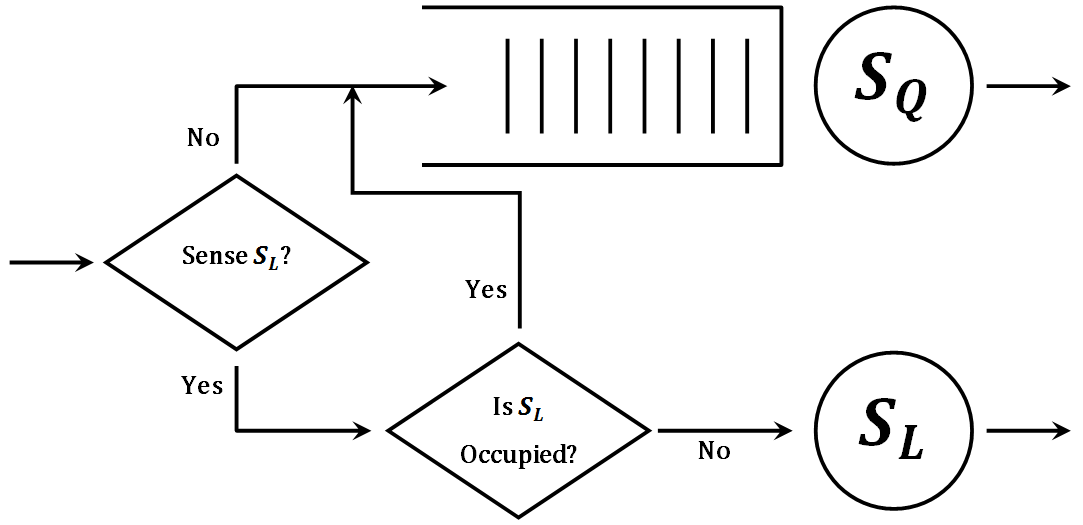
\includegraphics[width=1\textwidth]{plots/Model.png}
    \caption{Customers' flow chart of the system with an opportunistic sensing}
    \label{CustomersFlow}
\end{figure}

\begin{figure}[h!]
  \centering
    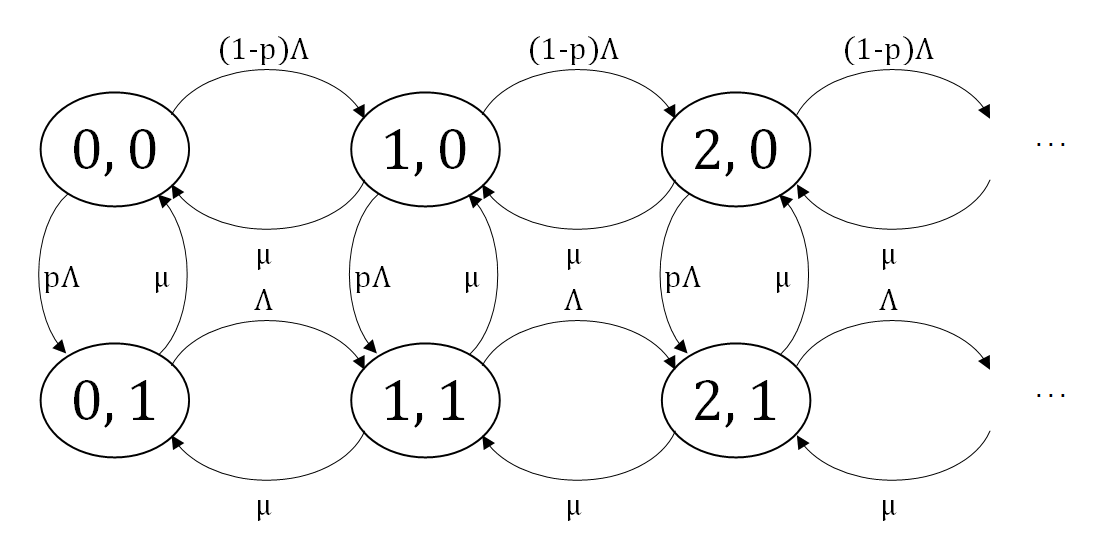
\includegraphics[width=1\textwidth]{plots/MarkovChain.png}
    \caption{The Markov chain describing the transitions between states in the system}
    \label{MarkovChain}
\end{figure}

\newpage
\begin{figure}[h!]
  \centering
    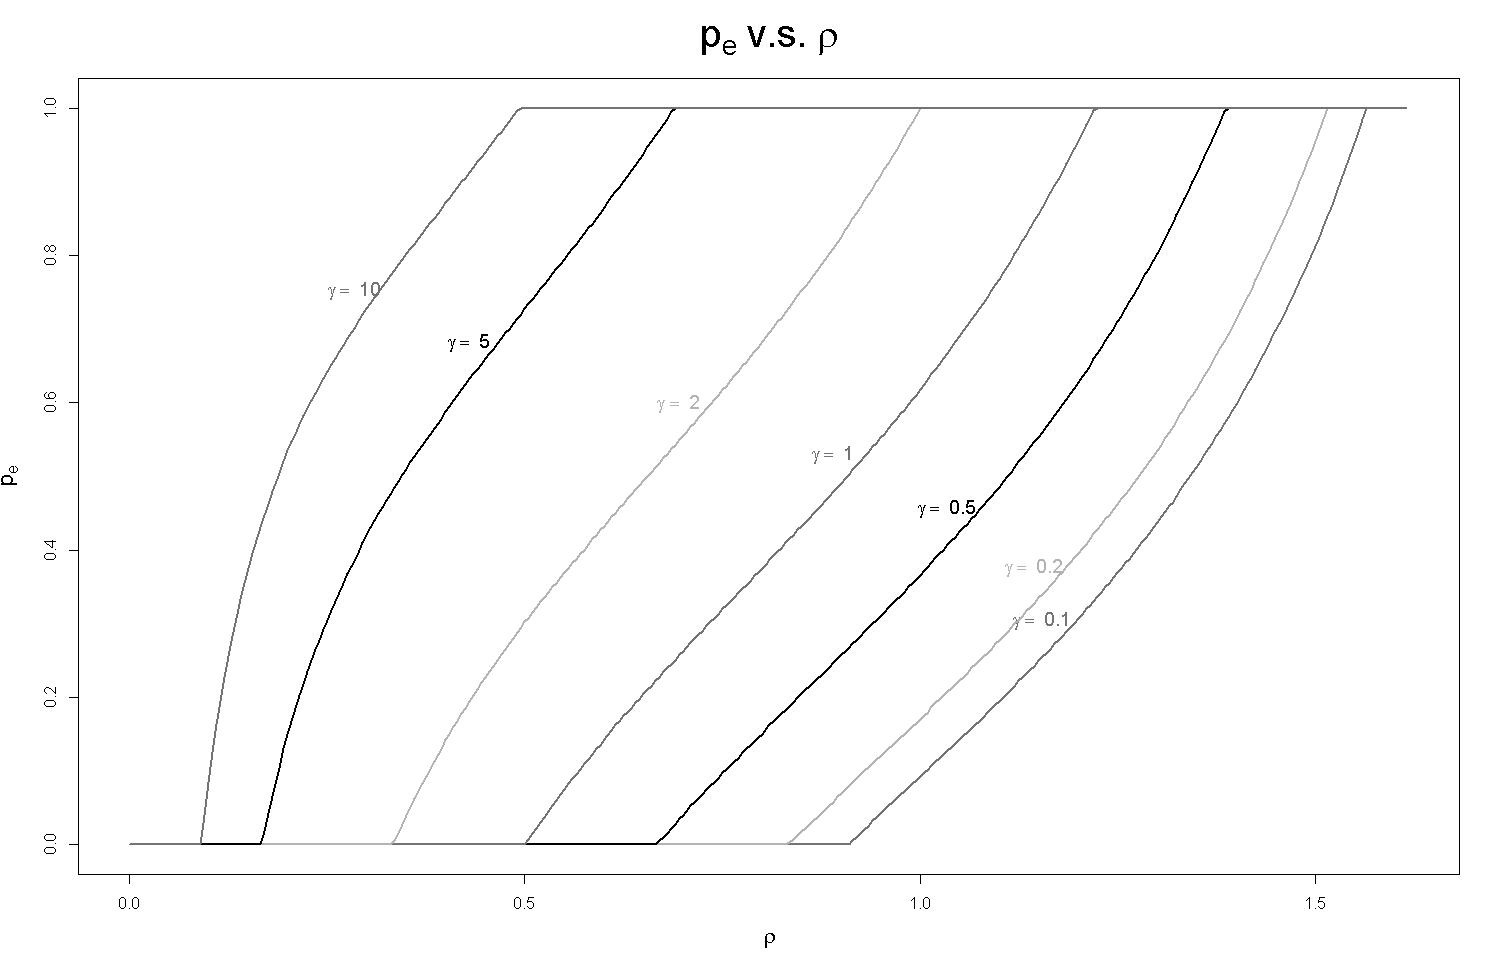
\includegraphics[width=1\textwidth]{plots/peq_vs_rho.png}
    \caption{The equilibrium strategy $p_{e}$ as a function of $\rho$ for a various values of $\gamma$}
    \label{PeqVsRho}
\end{figure}

\newpage
\begin{figure}[h!]
	\centering
	\begin{subfigure}[b]{0.49\textwidth}
	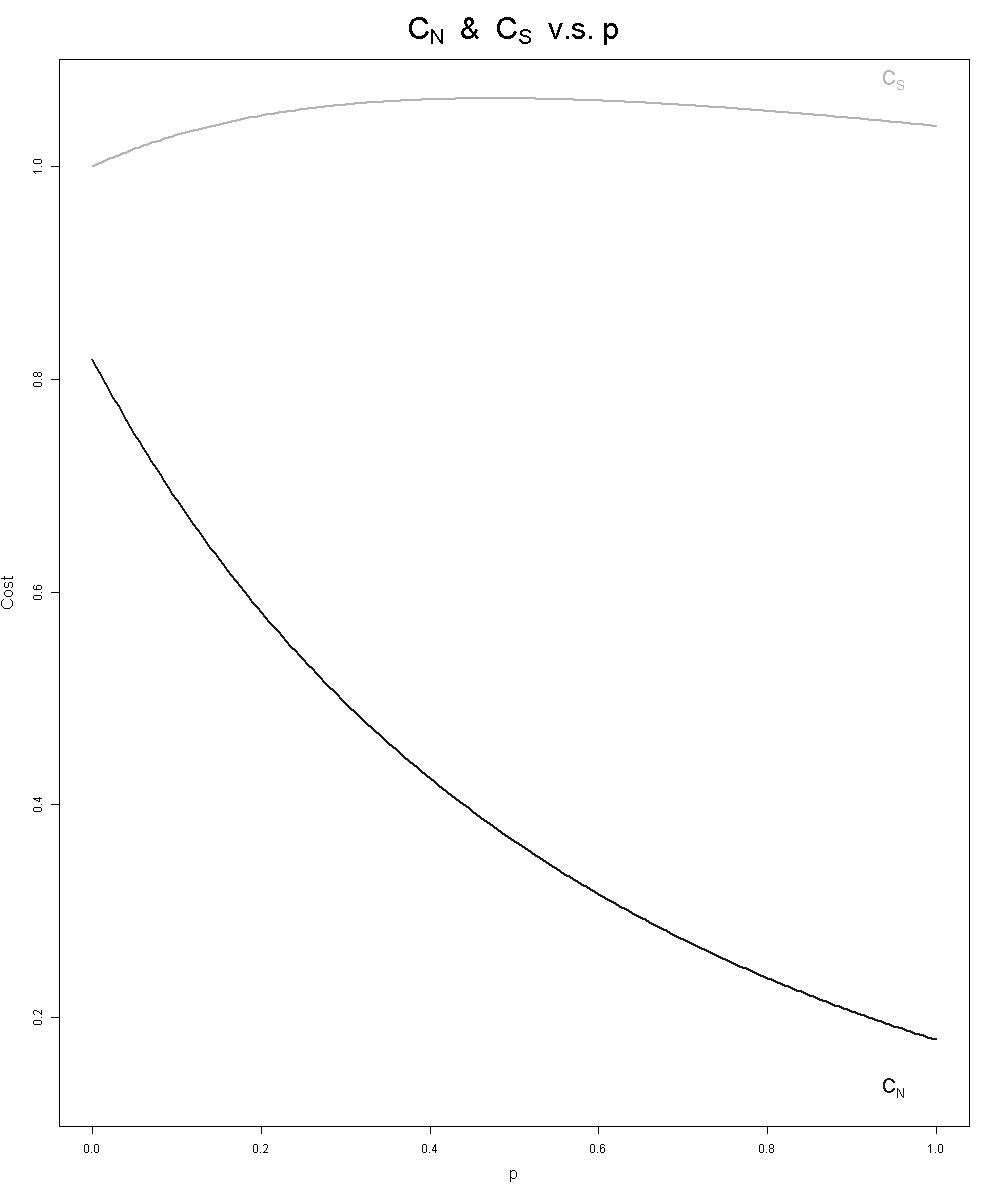
\includegraphics[width=\textwidth]{plots/cost_vs_p_1_0_45.png}
	\caption{$\gamma=1;\quad\rho=0.45$}
	\label{cost_vs_p_1_0_45}
	\end{subfigure}
	\begin{subfigure}[b]{0.49\textwidth}
	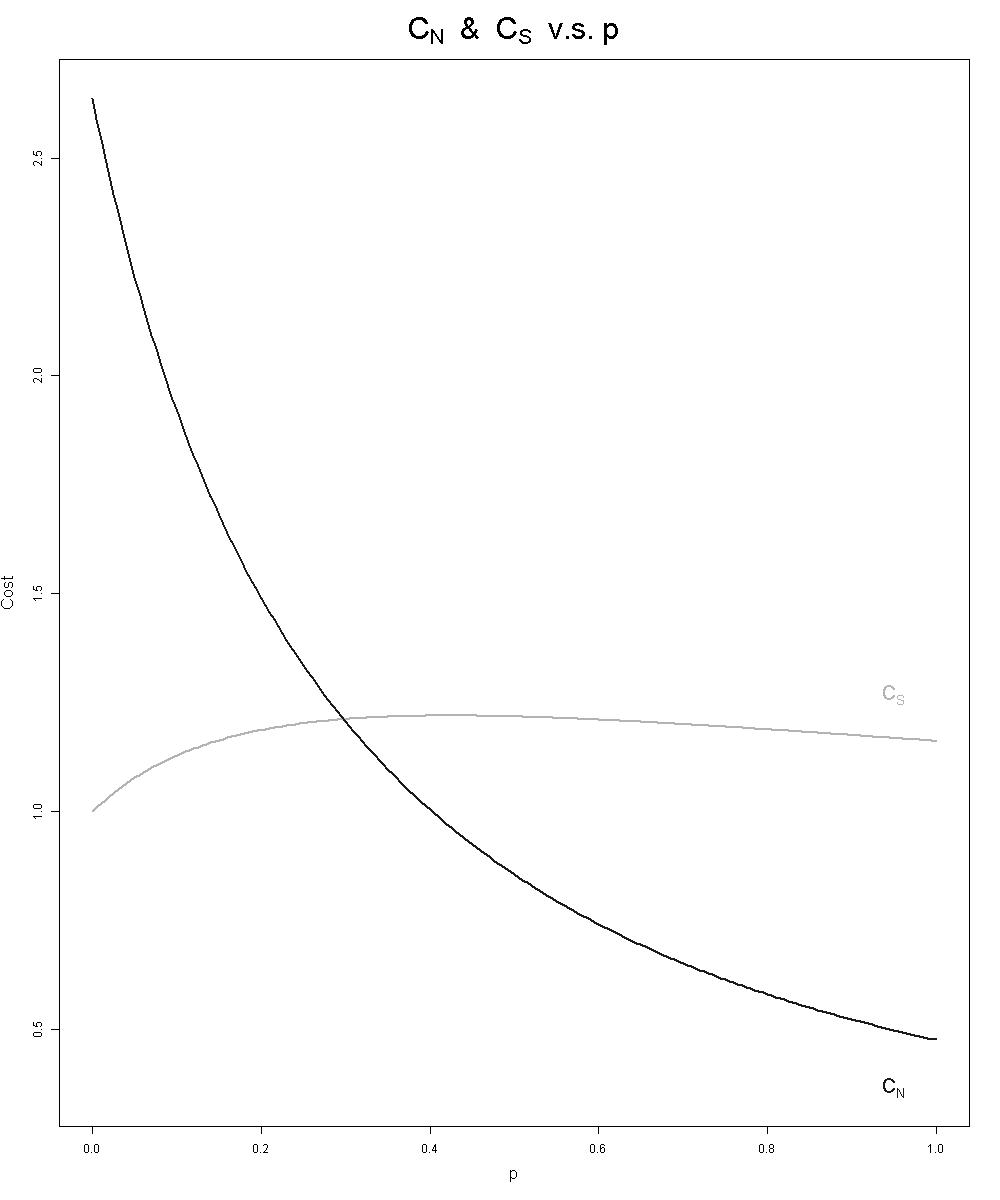
\includegraphics[width=\textwidth]{plots/cost_vs_p_1_0_725.png}
		\caption{$\gamma=1;\quad\rho=0.725$}
		\label{cost_vs_p_1_0_725}
	\end{subfigure}
          
	\begin{subfigure}[b]{0.49\textwidth}
	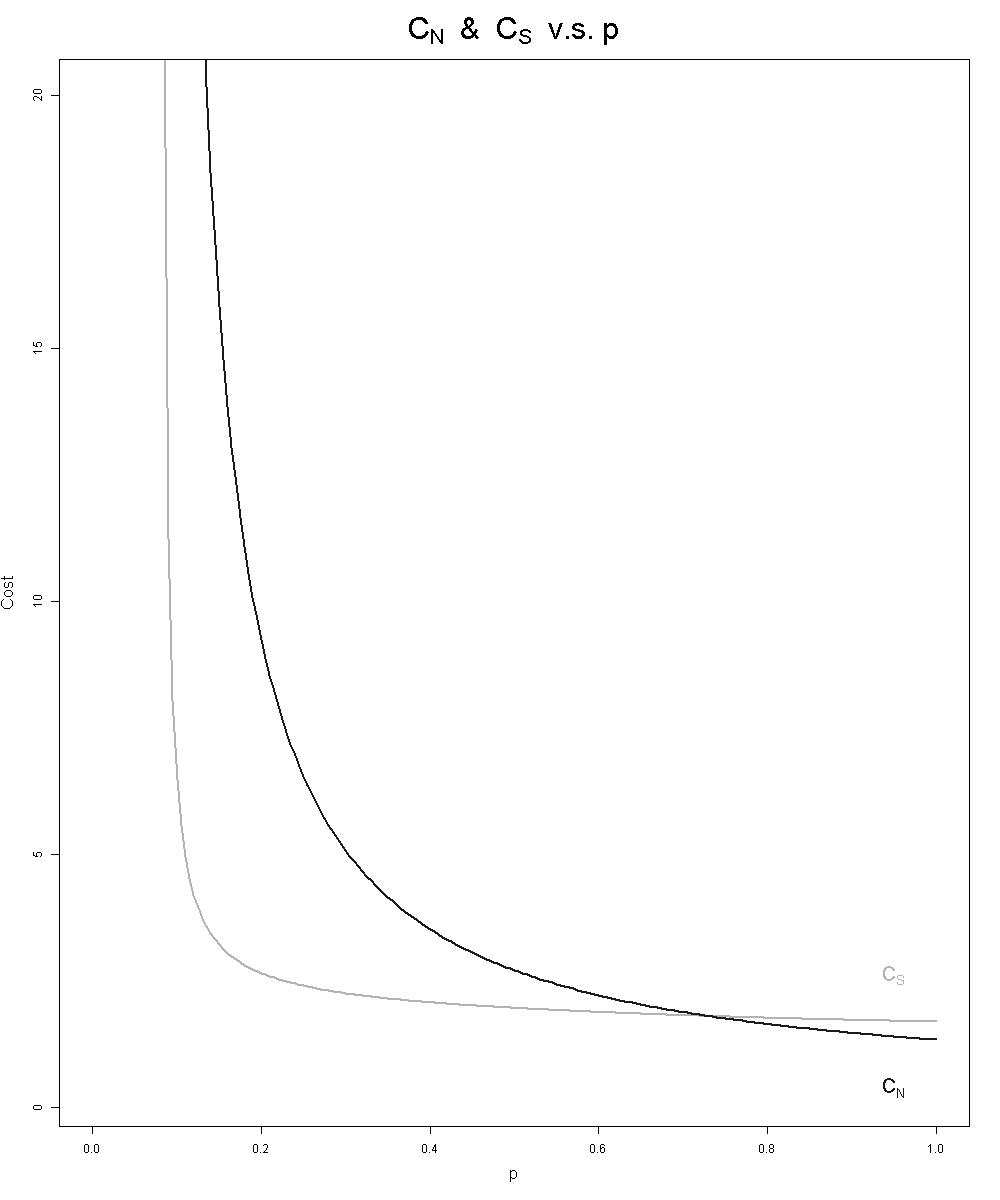
\includegraphics[width=\textwidth]{plots/cost_vs_p_1_1_08.png}
		\caption{$\gamma=1;\quad\rho=1.08$}
		\label{cost_vs_p_1_1_08}
	\end{subfigure}
	\begin{subfigure}[b]{0.49\textwidth}
	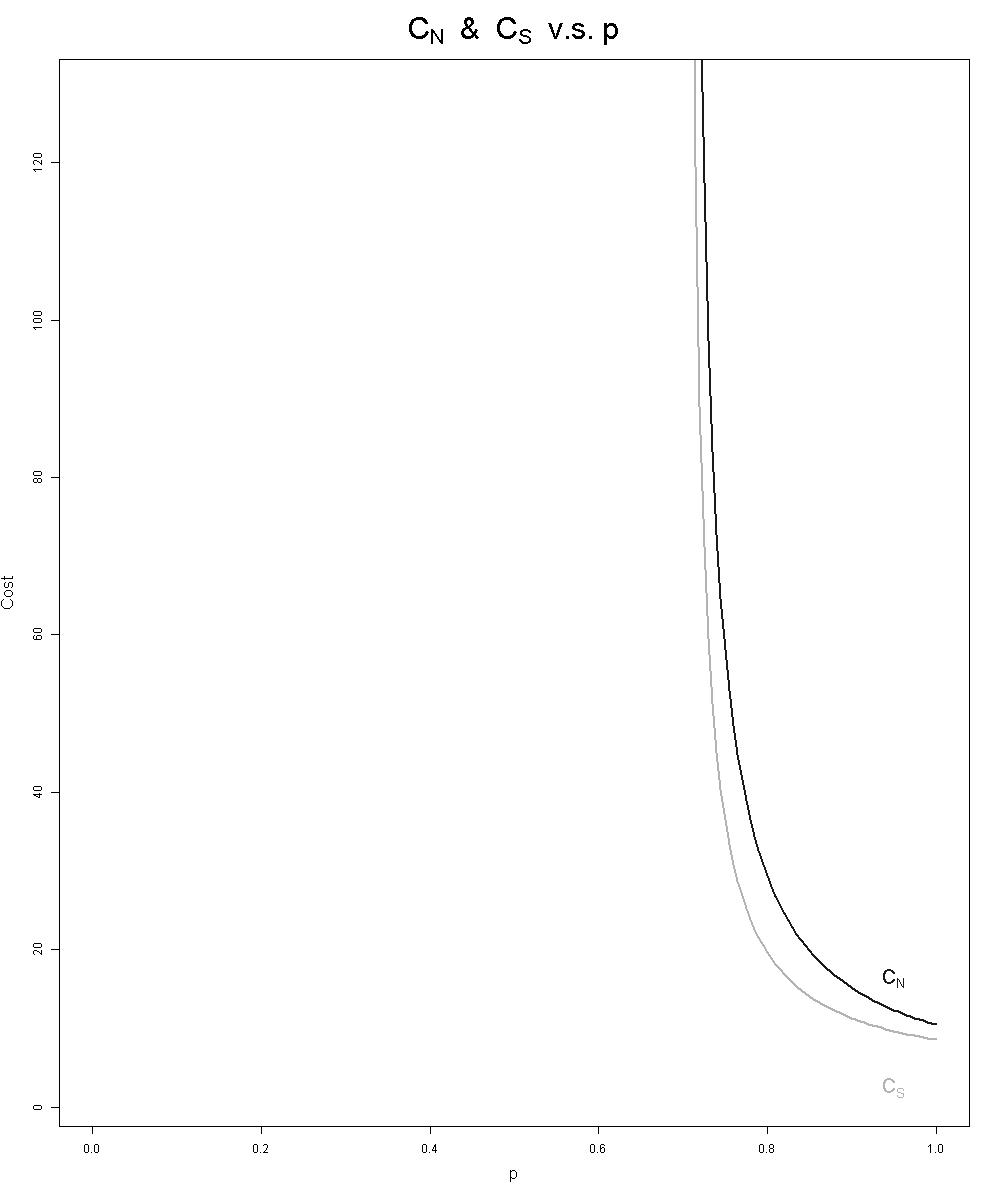
\includegraphics[width=\textwidth]{plots/cost_vs_p_1_1_515.png}
		\caption{$\gamma=1;\quad\rho=1.515$}
		\label{cost_vs_p_1_1_515}
	\end{subfigure}
	\caption{The expected costs of sensing and not sensing as a function of $p$ cosidering $\gamma=1$ and various values of $\rho$.}\label{CostVsP gamma=1}
\end{figure}

\newpage
\begin{figure}[h!]
	\centering
	\begin{subfigure}[b]{0.49\textwidth}
	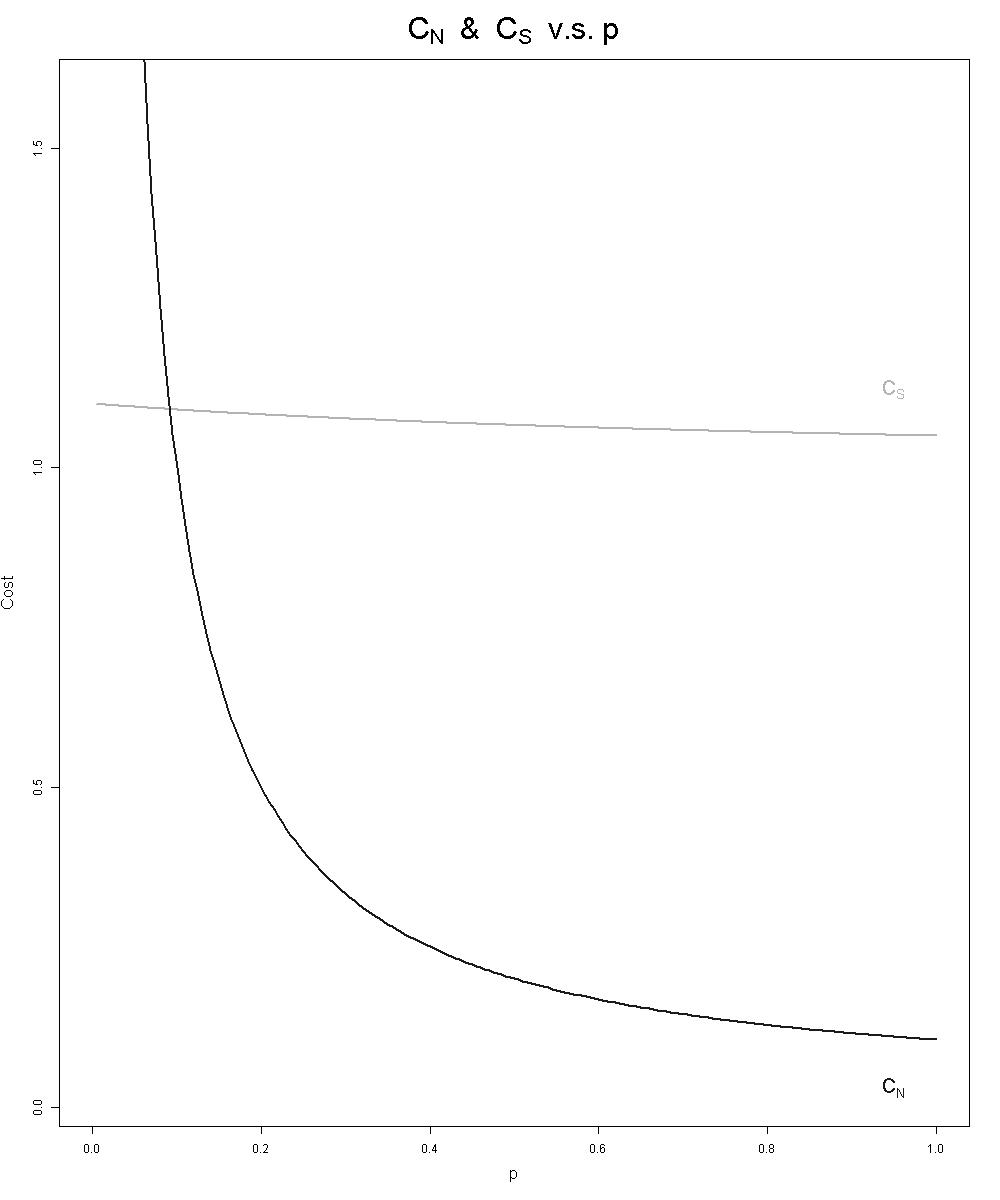
\includegraphics[width=\textwidth]{plots/cost_vs_p_0_1_1.png}
		\caption{$\gamma=0.1;\quad\rho=1$}
		\label{cost_vs_p_0_1_1}
	\end{subfigure}
	\begin{subfigure}[b]{0.49\textwidth}
	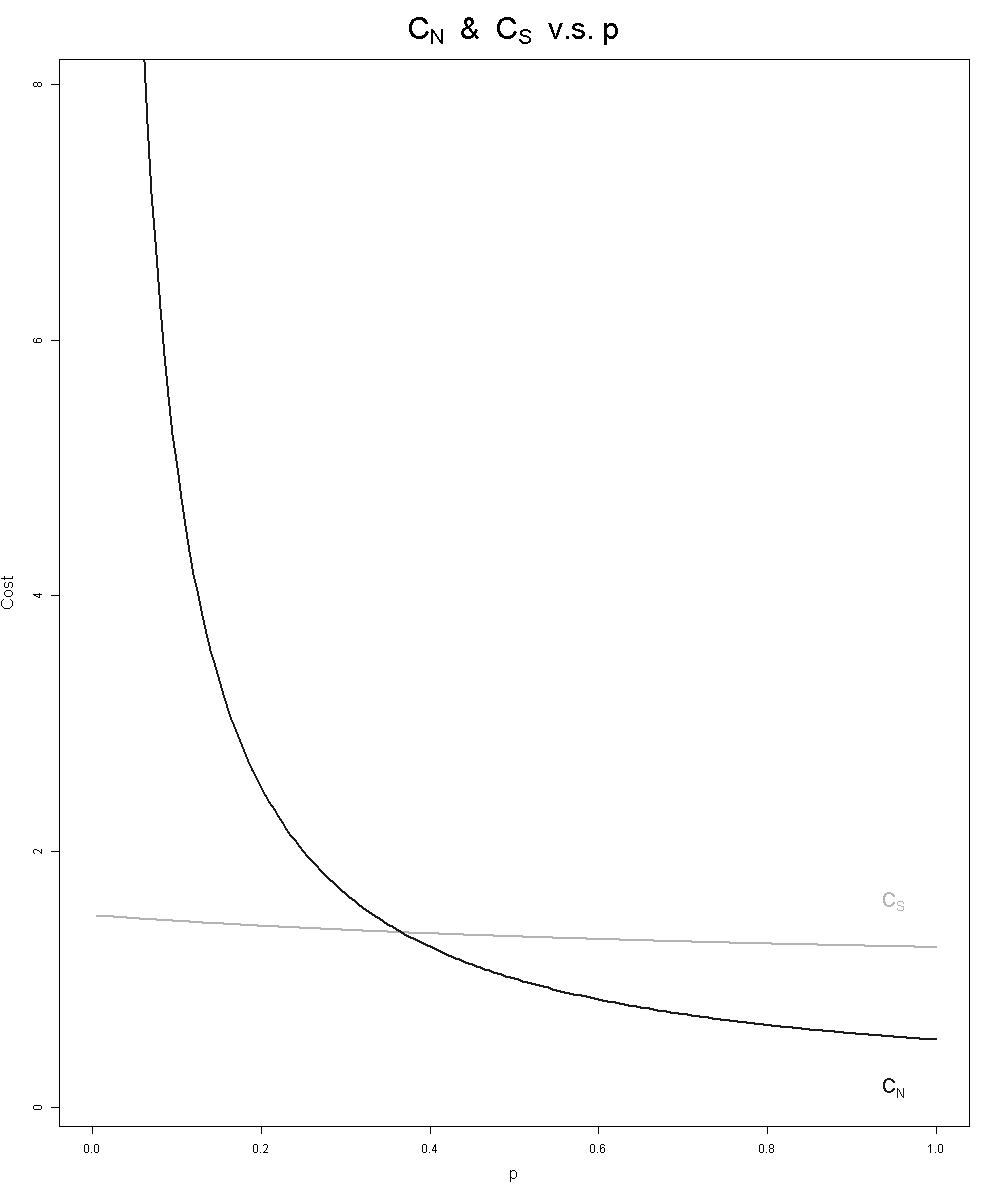
\includegraphics[width=\textwidth]{plots/cost_vs_p_0_5_1.png}
		\caption{$\gamma=0.5;\quad\rho=1$}
		\label{cost_vs_p_0_5_1}
	\end{subfigure}       
	\begin{subfigure}[b]{0.49\textwidth}
	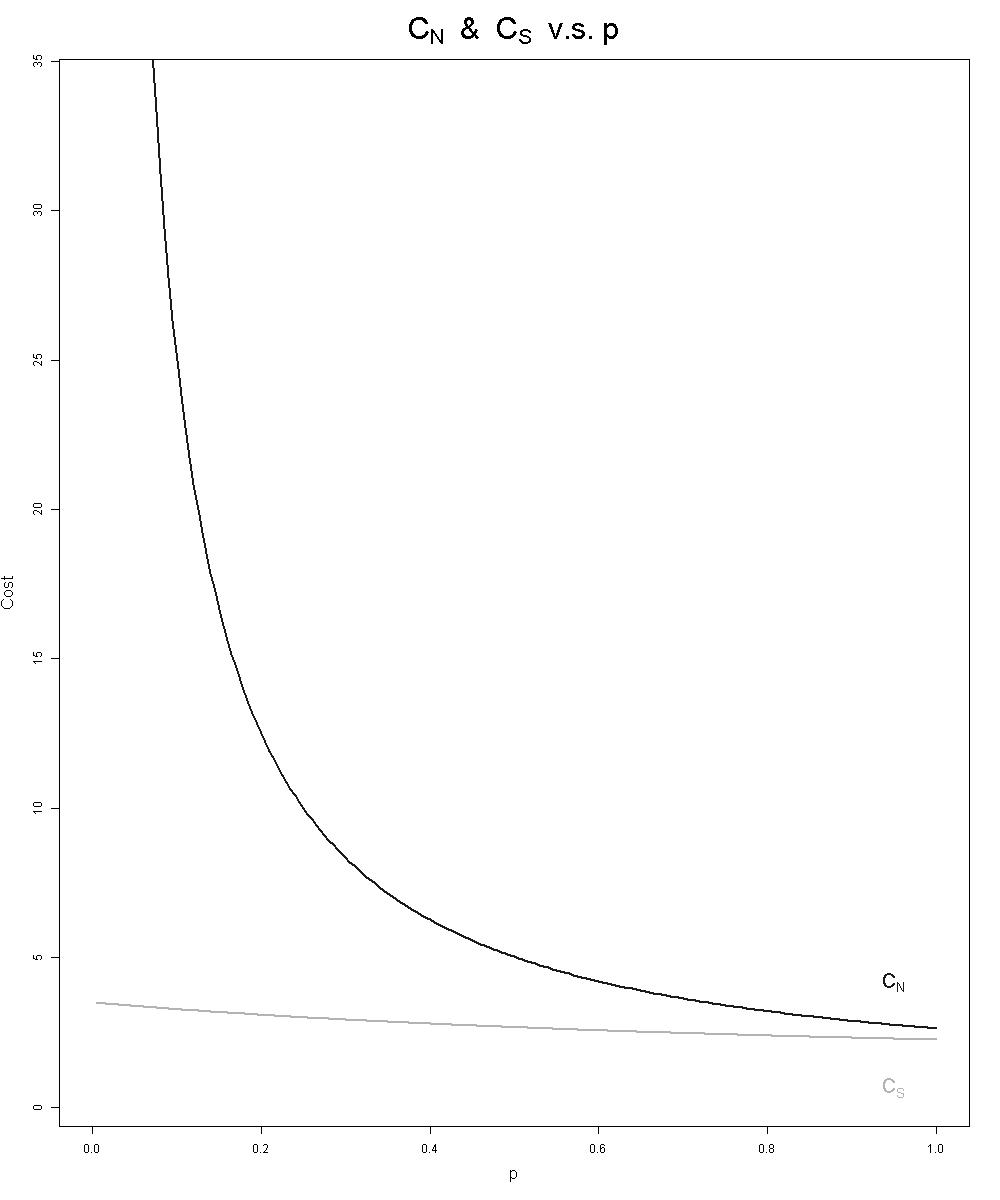
\includegraphics[width=\textwidth]{plots/cost_vs_p_2_5_1.png}
		\caption{$\gamma=2.5;\quad\rho=1$}
		\label{cost_vs_p_2_5_1}
	\end{subfigure}
	\begin{subfigure}[b]{0.49\textwidth}
	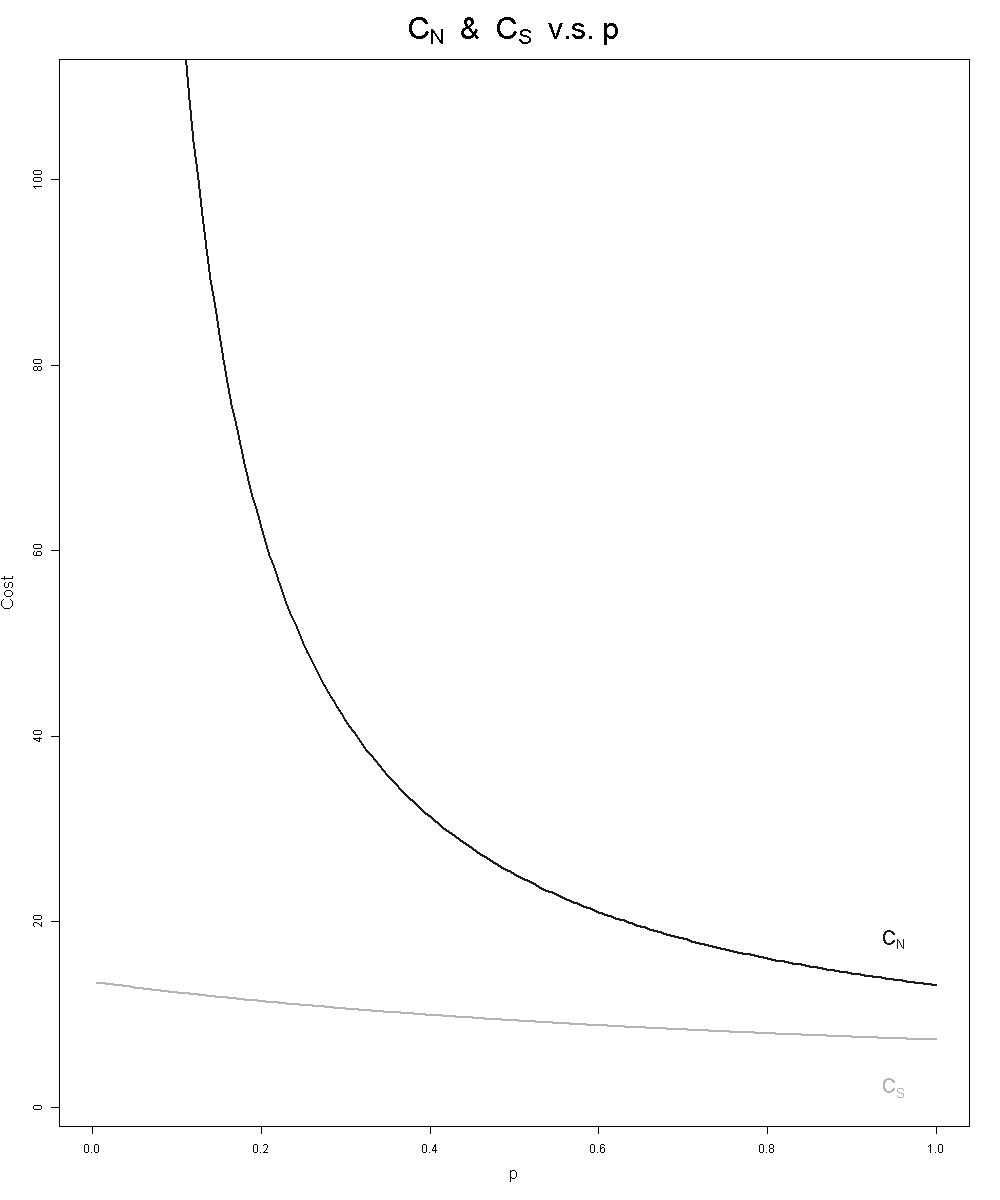
\includegraphics[width=\textwidth]{plots/cost_vs_p_12_5_1.png}
		\caption{$\gamma=12.5;\quad\rho=1$}
		\label{cost_vs_p_12_5_1}
	\end{subfigure}
	\caption{The expected costs of sensing ($C_S$) and not sensing ($C_N$) as a function of $p$ cosidering $\rho=1$ and various values of $\gamma$.}\label{CostVsP rho=1}
\end{figure}

\newpage
\begin{figure}[h!]
	\centering
	\begin{subfigure}[b]{0.49\textwidth}
	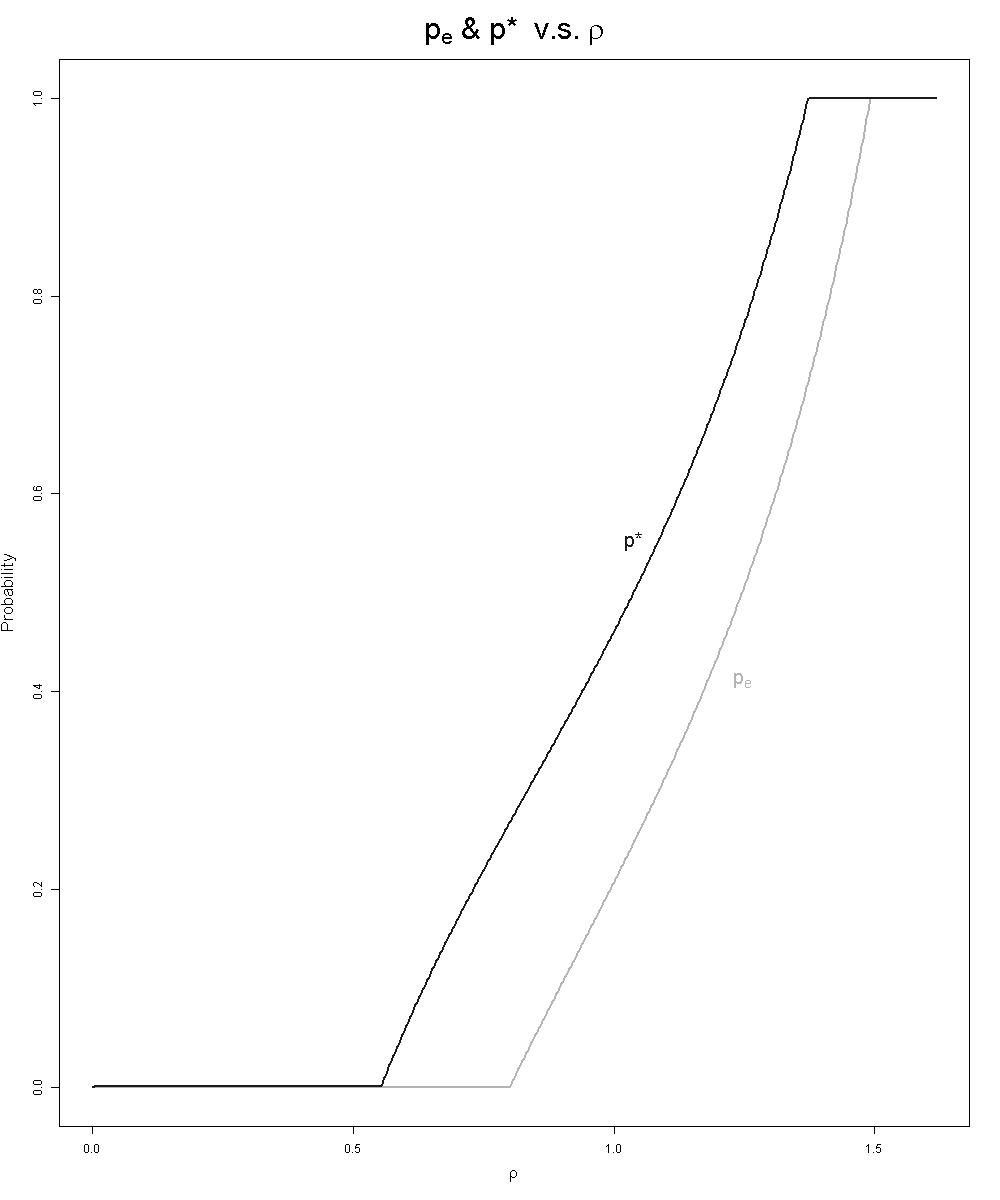
\includegraphics[width=\textwidth]{plots/pe_vs_pstar_0_25.png}
		\caption{$\gamma=0.25$}
	\end{subfigure}
	\begin{subfigure}[b]{0.49\textwidth}
	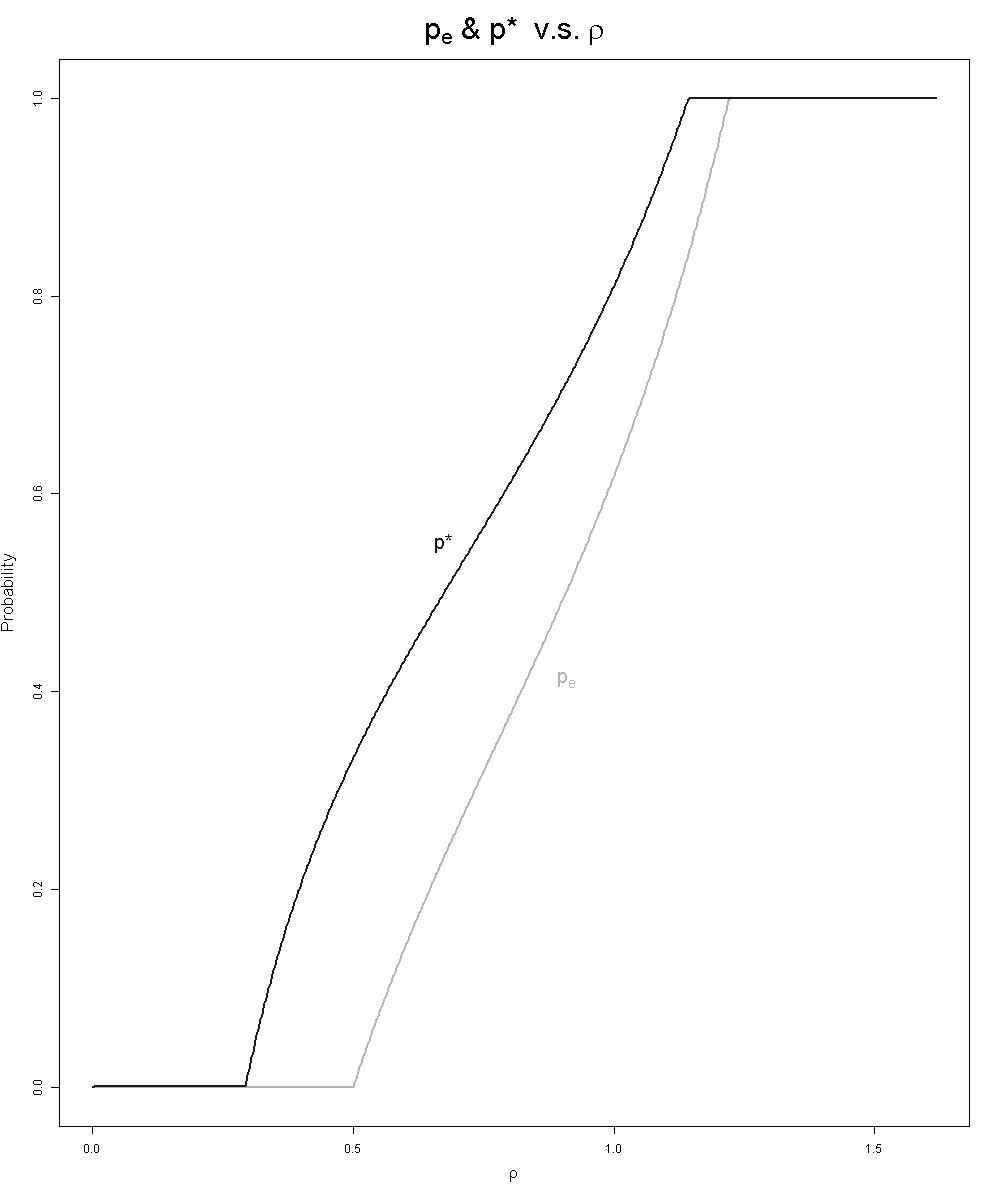
\includegraphics[width=\textwidth]{plots/pe_vs_pstar_1.png}
		\caption{$\gamma=1$}
	\end{subfigure}
	\begin{subfigure}[b]{0.49\textwidth}
	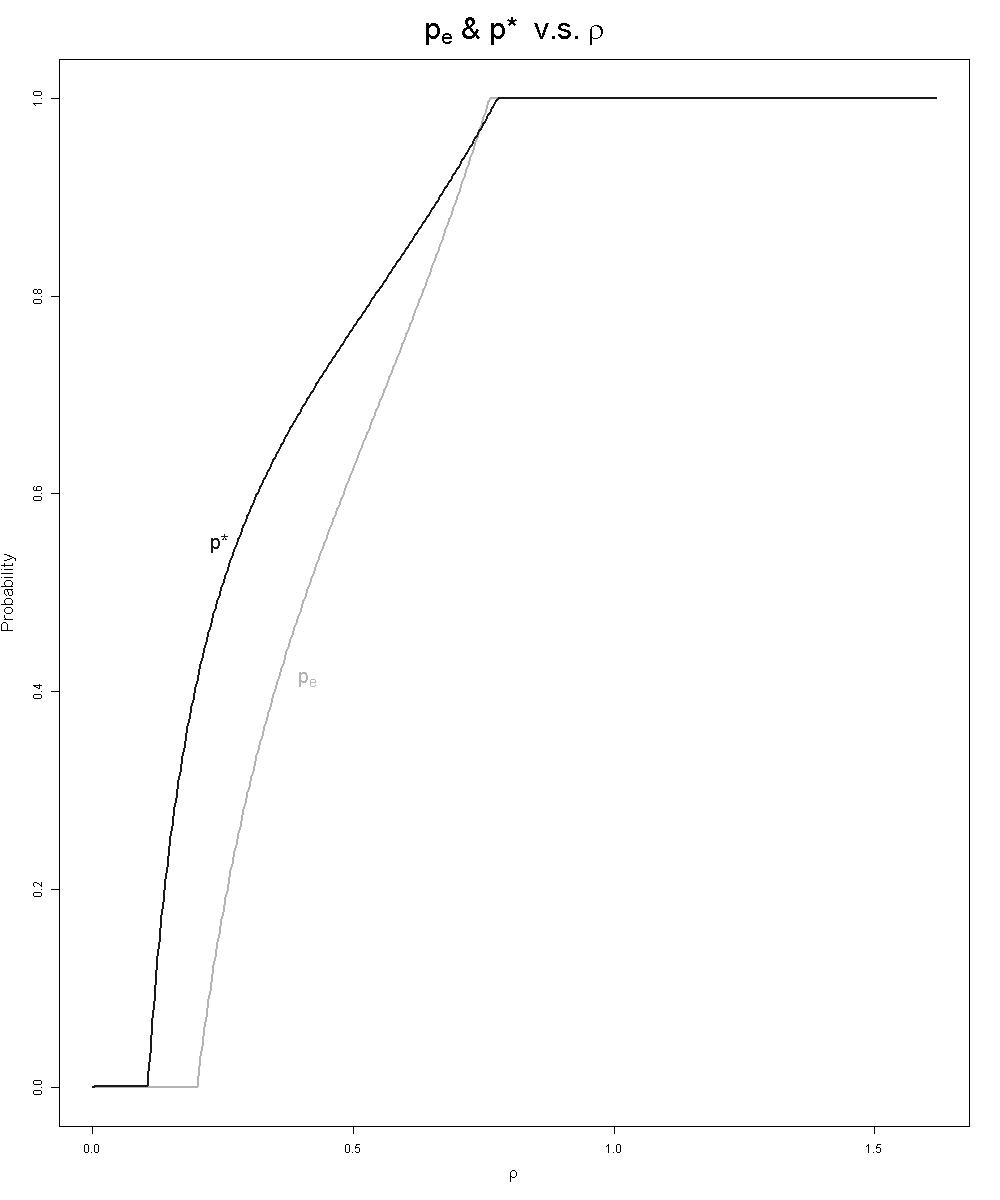
\includegraphics[width=\textwidth]{plots/pe_vs_pstar_4.png}
		\caption{$\gamma=4$}
	\end{subfigure}
	\begin{subfigure}[b]{0.49\textwidth}
	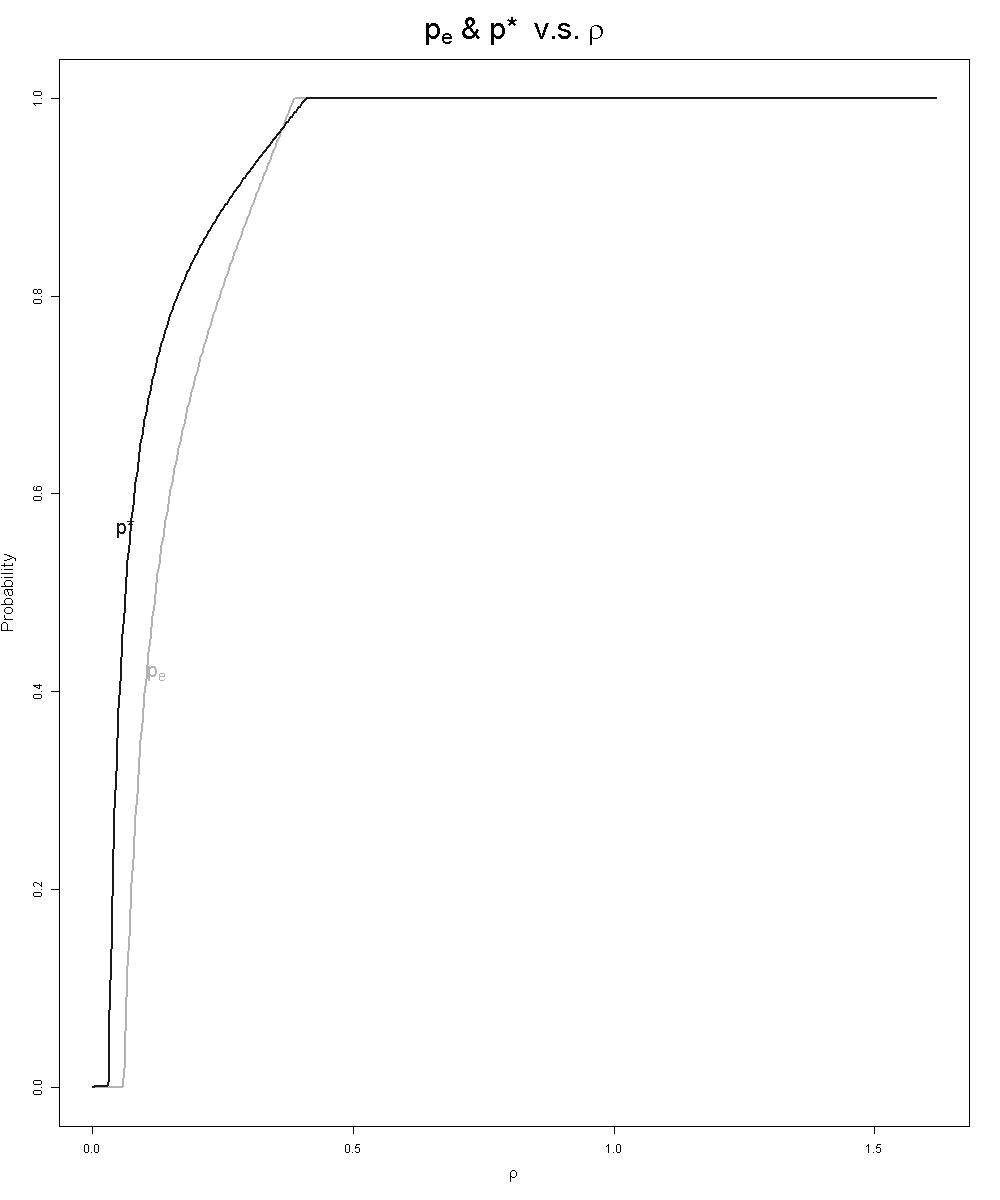
\includegraphics[width=\textwidth]{plots/pe_vs_pstar_16.png}
		\caption{$\gamma=16$}
	\end{subfigure}
	\caption{The socially optimal strategy ($p^*$) and the equilibrium strategy ($p_e$) as a function of $\rho$ cosidering various values values of $\gamma$.}\label{p_e and p*}
\end{figure}

\newpage
\begin{figure}[h!]
	\centering
	\begin{subfigure}[b]{0.49\textwidth}
	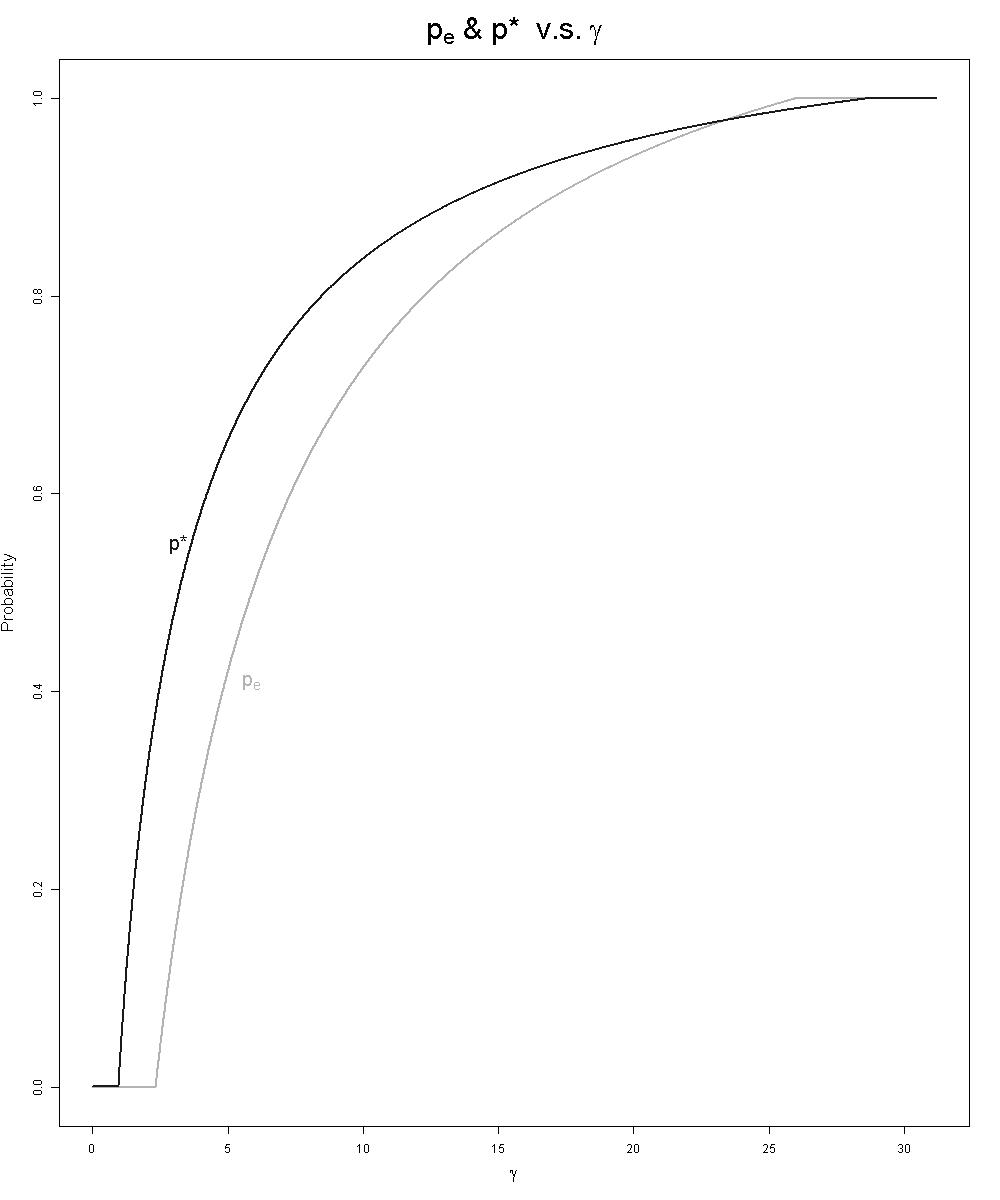
\includegraphics[width=\textwidth]{plots/pe_vs_pstar_rev_0_3.png}
		\caption{$\rho=0.3$}
	\end{subfigure}
	\begin{subfigure}[b]{0.49\textwidth}
	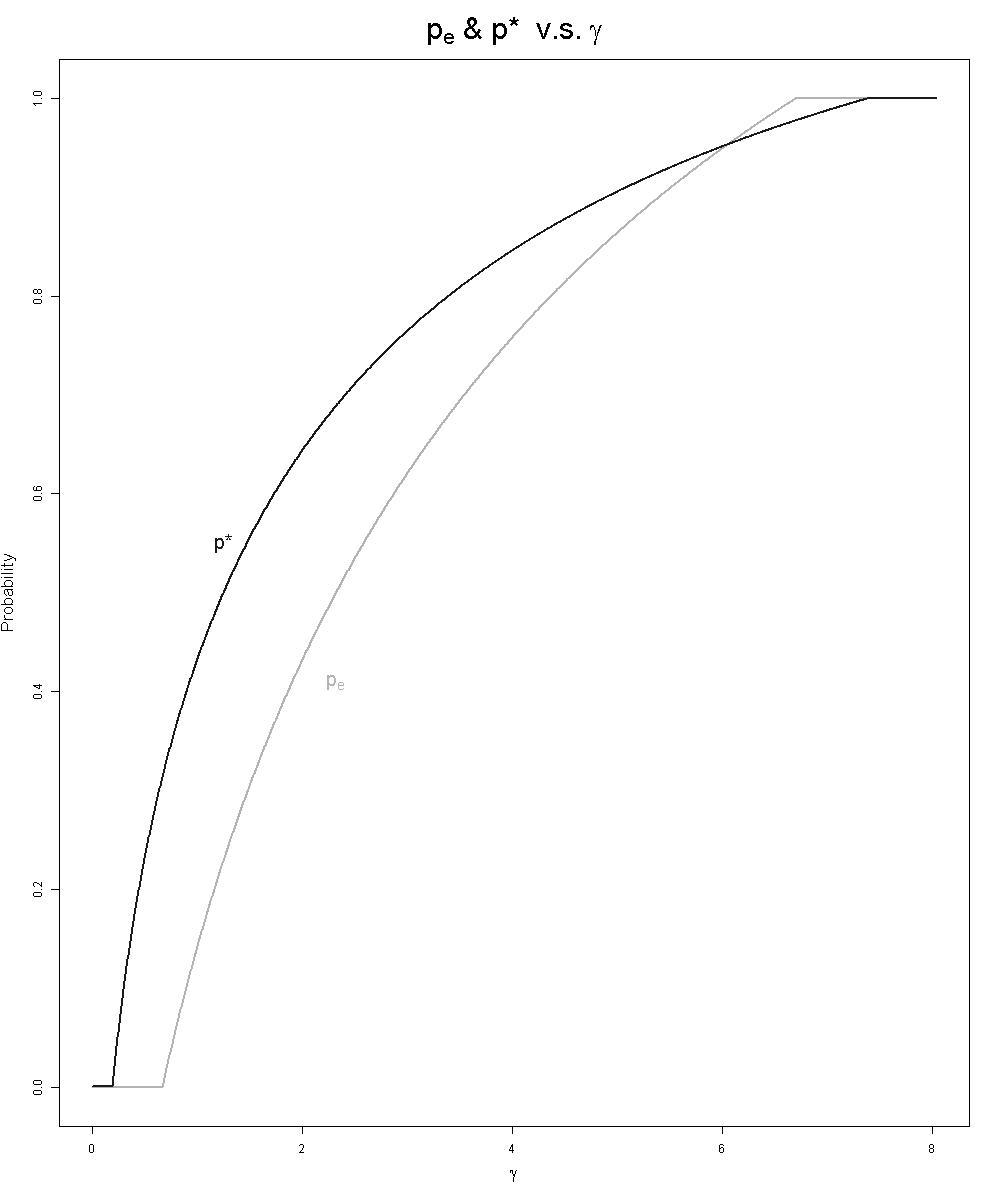
\includegraphics[width=\textwidth]{plots/pe_vs_pstar_rev_0_6.png}
		\caption{$\rho=0.6$}
	\end{subfigure}
	\begin{subfigure}[b]{0.49\textwidth}
	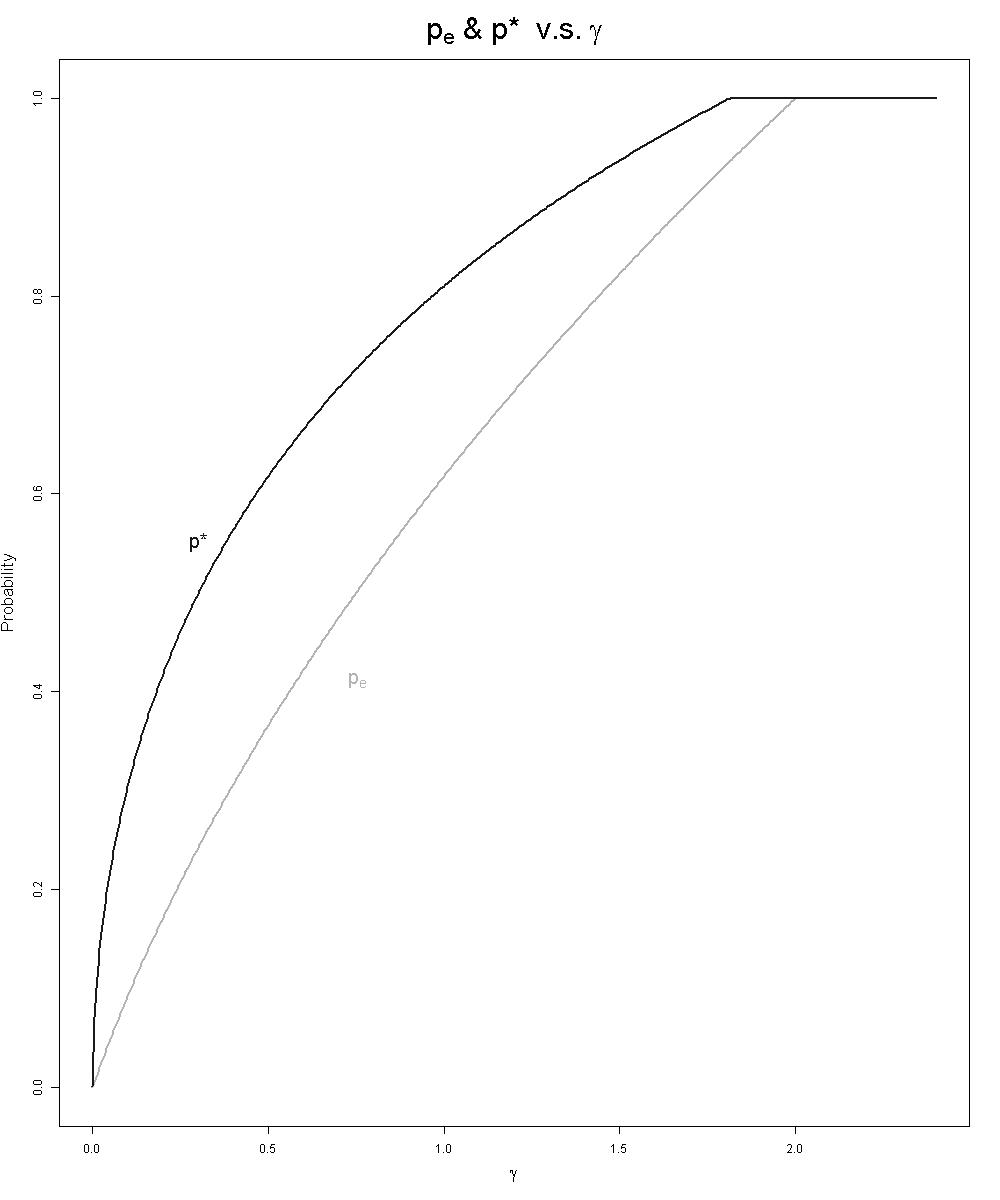
\includegraphics[width=\textwidth]{plots/pe_vs_pstar_rev_1.png}
		\caption{$\rho=1$}
	\end{subfigure}
	\begin{subfigure}[b]{0.49\textwidth}
	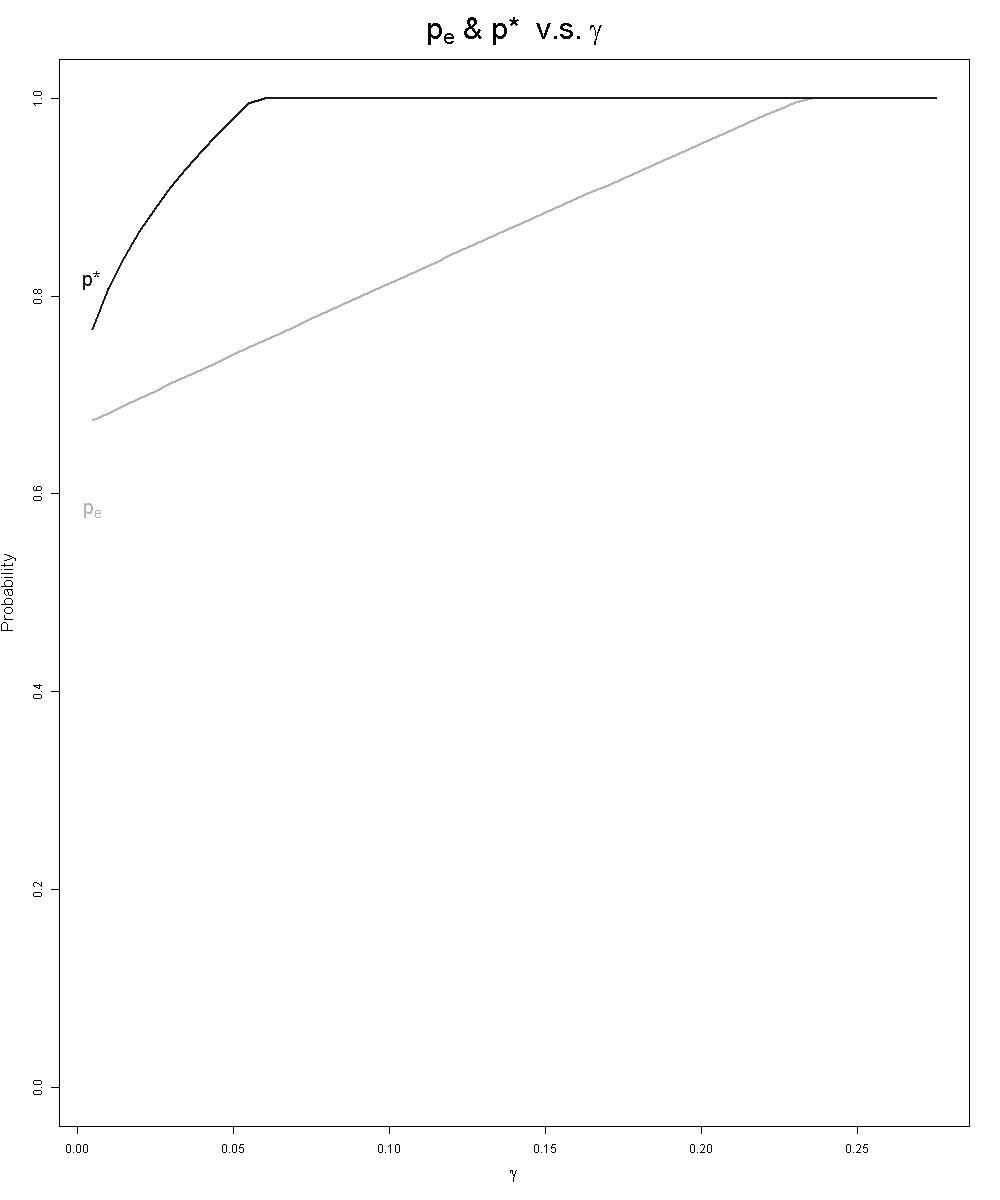
\includegraphics[width=\textwidth]{plots/pe_vs_pstar_rev_1_5.png}
		\caption{$\rho=1.5$}
	\end{subfigure}
	\caption{The socially optimal strategy ($p^*$) and the equilibrium strategy ($p_e$) as a function of $\gamma$ cosidering various values values of $\rho$.}\label{p_e and p*}
\end{figure}

\newpage
\begin{thebibliography}{99}

\bibitem{Do.C.T} Do, Chuong T., Nguyen H. Tran, Mui Van Nguyen, Choong Seon Hong and Sungwon Lee (2012) ``Social optimization strategy in unobserved queueing systems in cognitive radio networks,'' {\it IEEE Communications Letters}, Vol. 16,  pp. 1944-1947.

\bibitem{Habachi&Hayel} Habachi, Oussama and Yezekael Hayel (2012) ``Optimal opportunistic sensing in cognitive radio networks,'' {\it IET Communications}, Vol. 6, pp. 797-804. 

\bibitem{2QorNot2Q} Hassin, Refael and Moshe Haviv (2003) {\it To Queue or Not to Queue: Equilibrium Behavior in Queueing Systems}, Kluwer Academic Publishers, Boston.

\bibitem{Haykin} Haykin, Simon (2005) ``Cognitive radio: Brain-empowered wireless communications,'' {\it IEEE Journal on Selected Areas in Communications}, Vol. 23, pp. 201-220.

\bibitem{Yehiali&Naor} Yechiali, Uri and Pinhas Naor (1971) ``Queuing problems with heterogeneous arrivals and service,'' {\it Operations Research}, Vol. 19, pp. 722-734.

\end{thebibliography}

\end{document}
